%%%%%%%%%%%%%%%%%%%%%%%%%%%%%%%%%%%%%%%%%%%%%%%%%%%%%%%%%%%%%%%%%%%%%%%%
% Plantilla TFG/TFM
% Escuela Politécnica Superior de la Universidad de Alicante
% Realizado por: Jose Manuel Requena Plens
% Contacto: info@jmrplens.com / Telegram:@jmrplens
%%%%%%%%%%%%%%%%%%%%%%%%%%%%%%%%%%%%%%%%%%%%%%%%%%%%%%%%%%%%%%%%%%%%%%%%

\chapter{Anexo I - Dimensiones de los arrays de parches microstrip diseñados}
\label{anexo}


\section{Parche Simple @ 2 GHz}

\vfill
\begin{figure}[H]
   	 \centering
        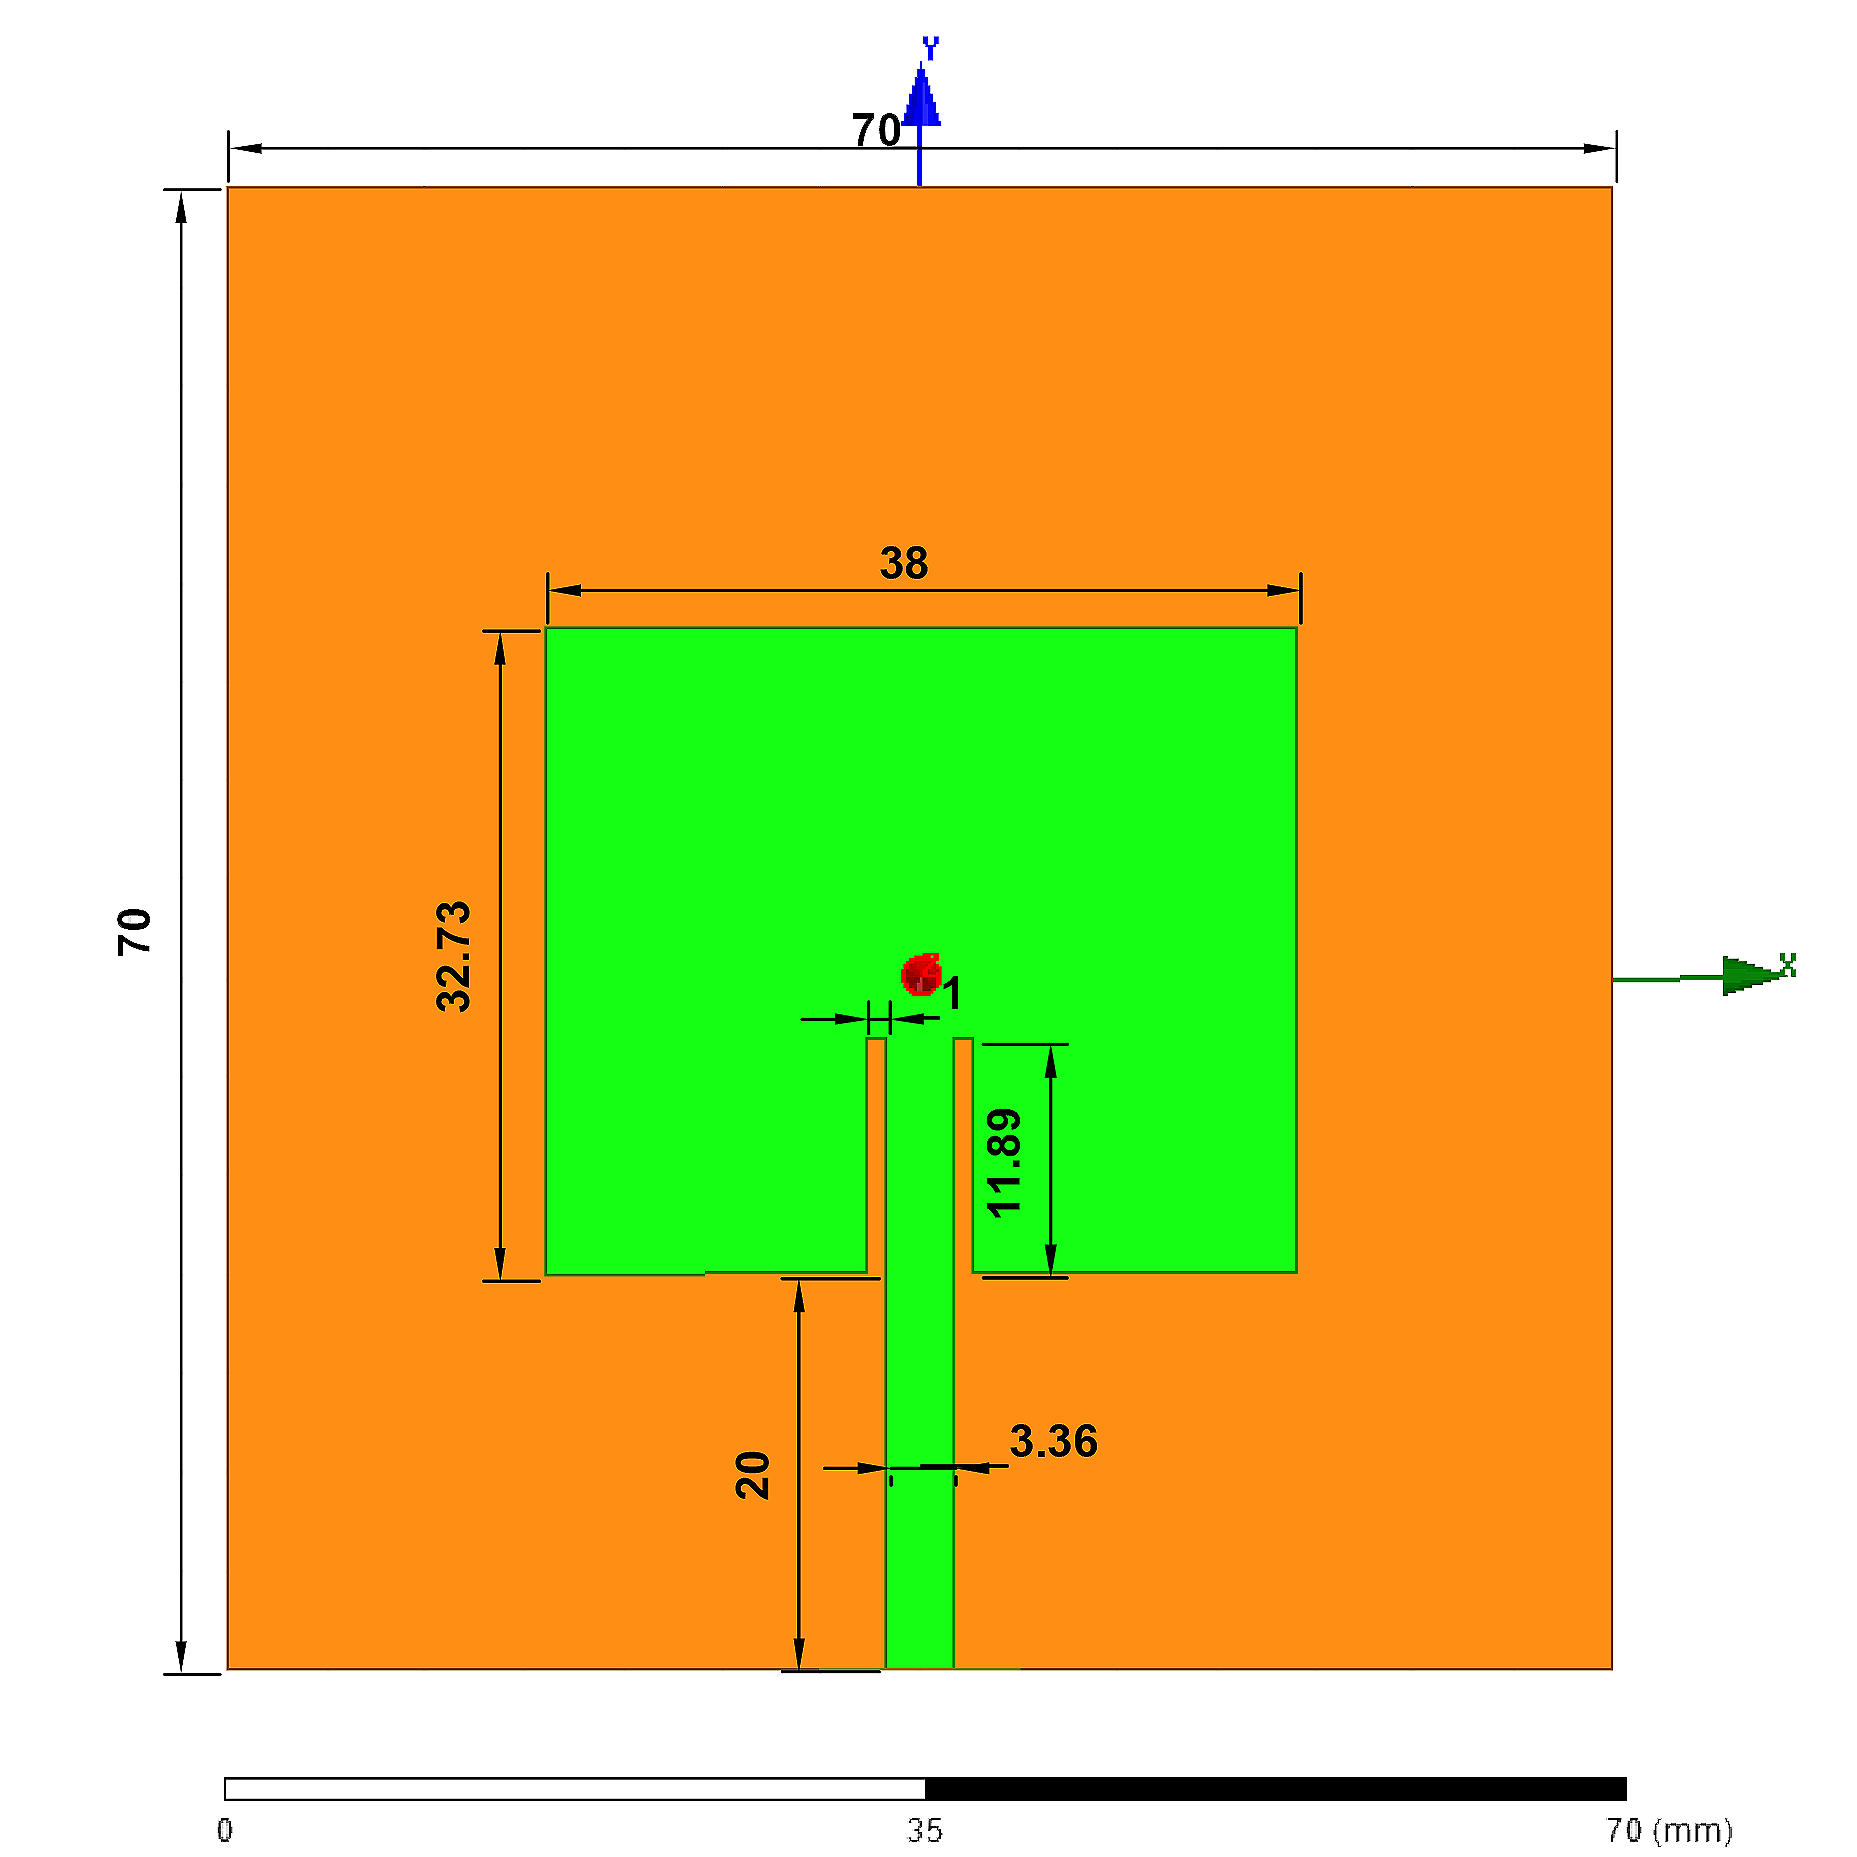
\includegraphics[width=\textwidth ,height=\textheight, keepaspectratio=true]{archivos/desarrollo/autocad/1}
        \caption{Dimensiones del parche simple a 2.4 GHz}
        \label{fig:simple1}
\end{figure}
\vfill
\textit{\textbf{Nota}}: todas las medidas están expresadas en milímetros.
\newpage


\section{Parche Simple @ 6 GHz}
\vfill
\begin{figure}[H]
   	 \centering
        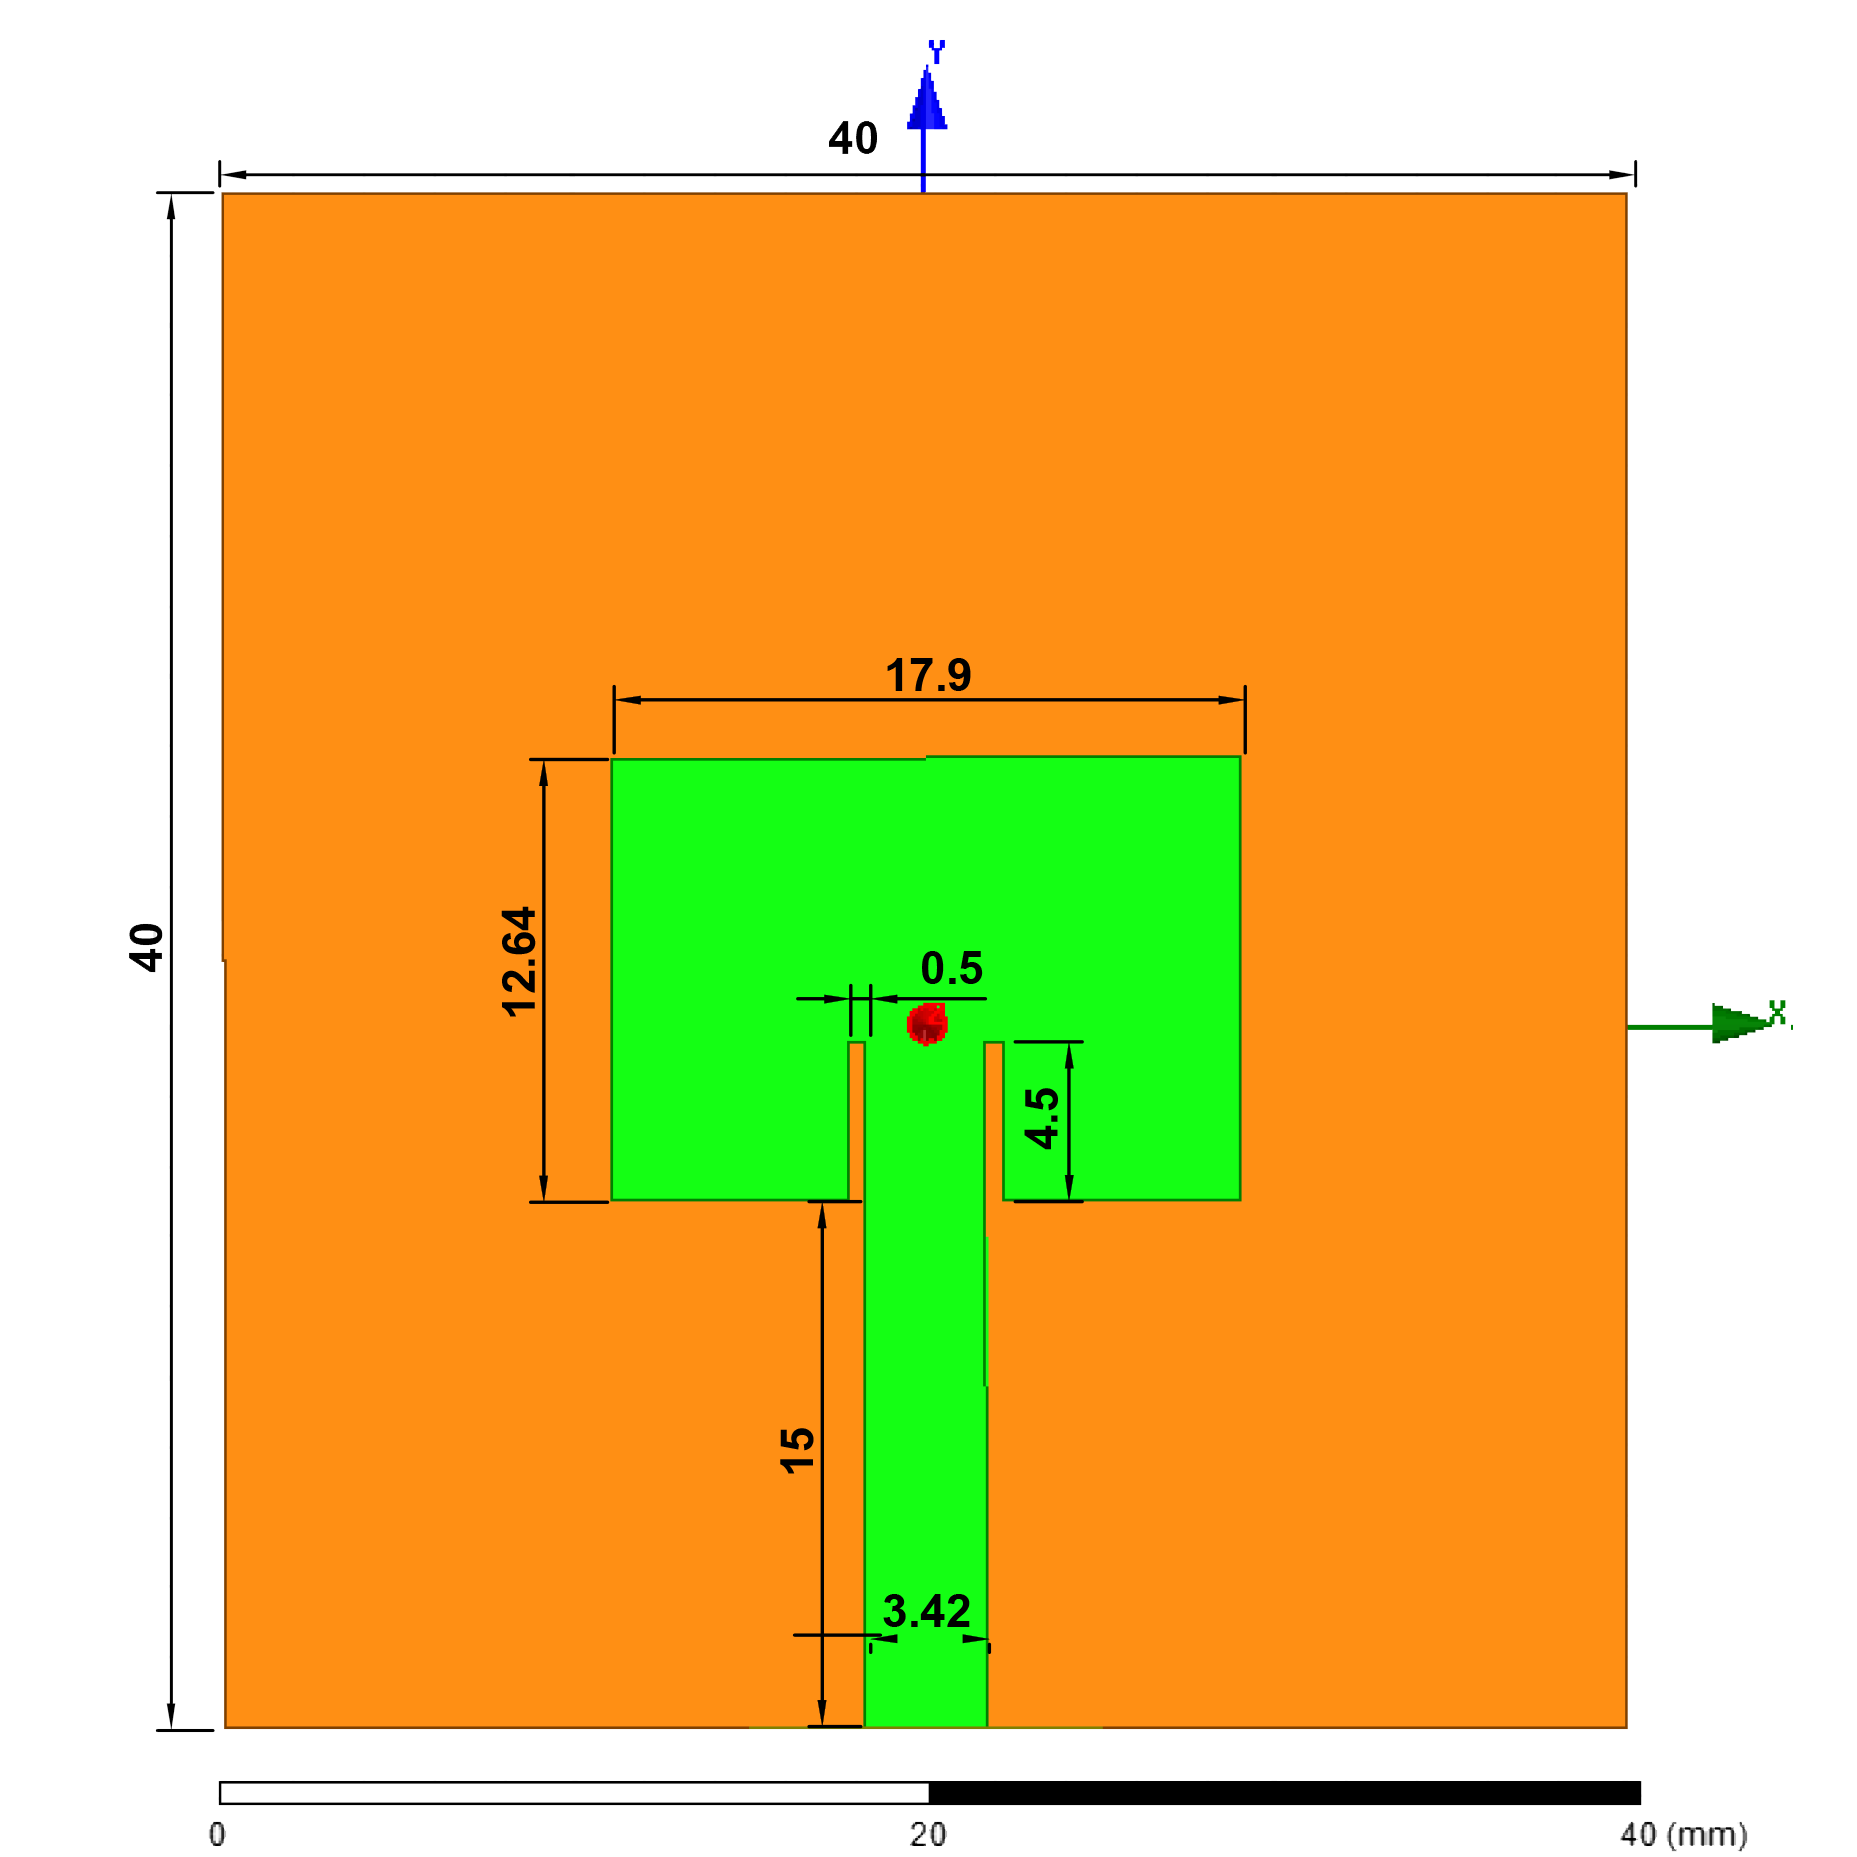
\includegraphics[width=\textwidth, height=\textheight, keepaspectratio=true]{archivos/desarrollo/autocad/2}
        \caption{Dimensiones del parche simple a 6 GHz}
        \label{fig:simple2}
\end{figure}

\vfill
\textit{\textbf{Nota}}: todas las medidas están expresadas en milímetros.
\newpage

\section{Array 2x1 @ 2.4 GHz}
\vfill
\begin{figure}[H]
   	 \centering
        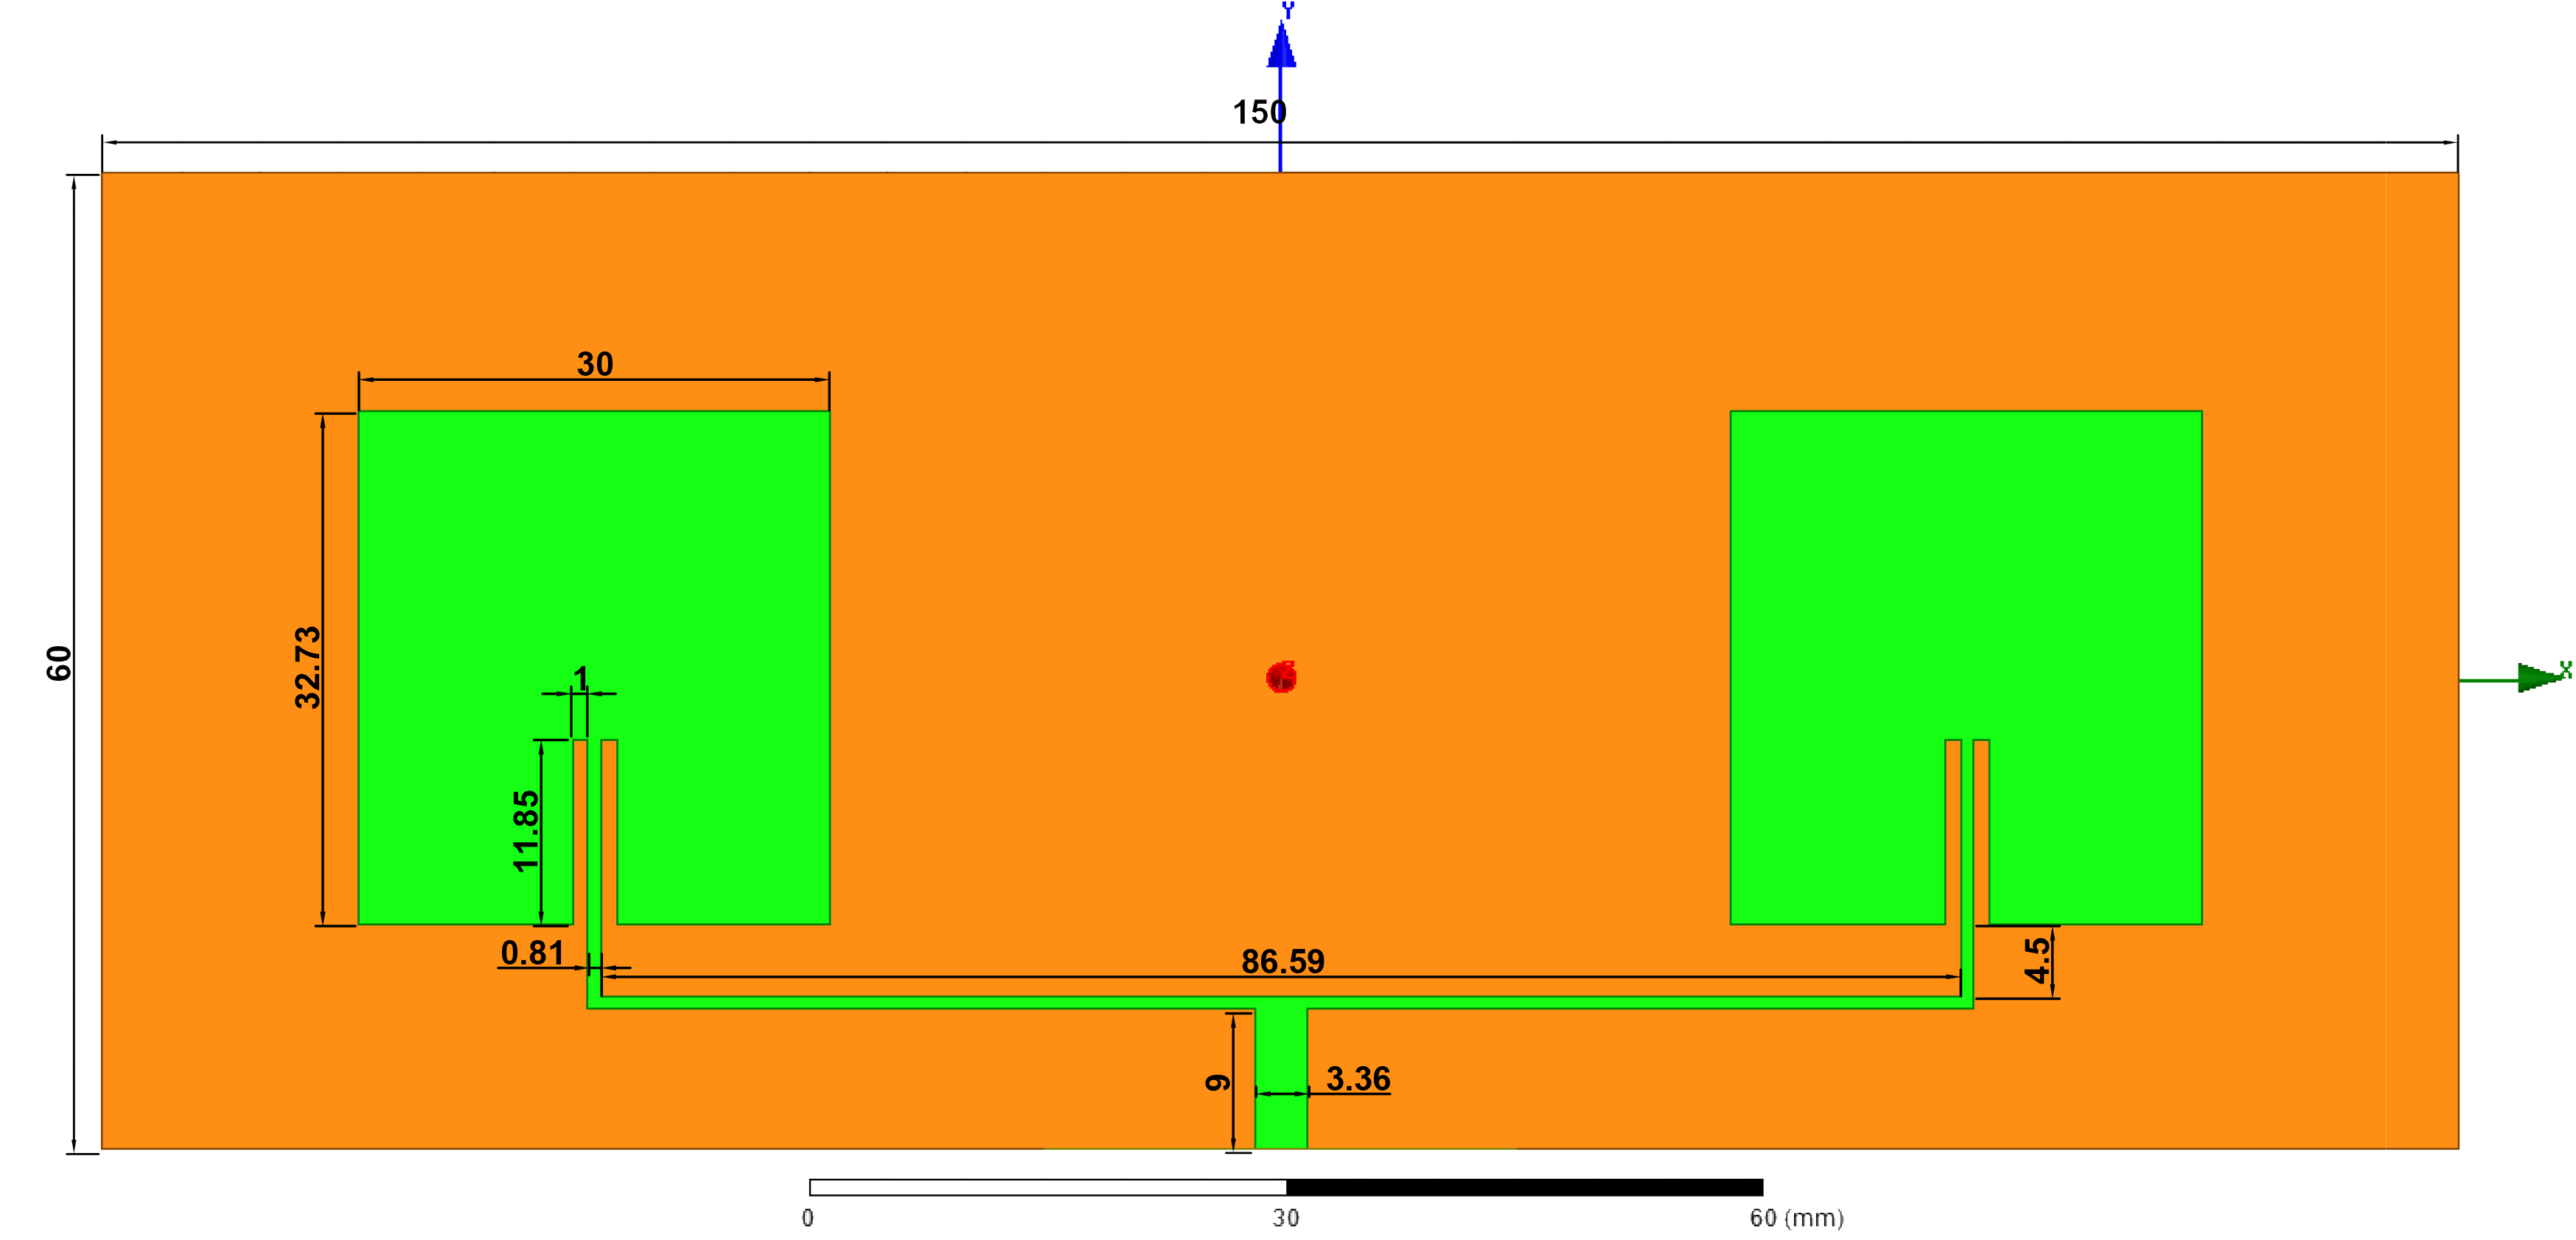
\includegraphics[width=18cm ,height=\textwidth, keepaspectratio=true,angle=90,origin=c]{archivos/desarrollo/autocad/3}
        \caption{Dimensiones del array 2x1 a 2.4 GHz}
        \label{fig:2x11}
\end{figure}
\vfill
\textit{\textbf{Nota}}: todas las medidas están expresadas en milímetros.
\newpage

\section{Array 2x1 @ 6 GHz}
\vfill
\begin{figure}[H]
   	 \centering
        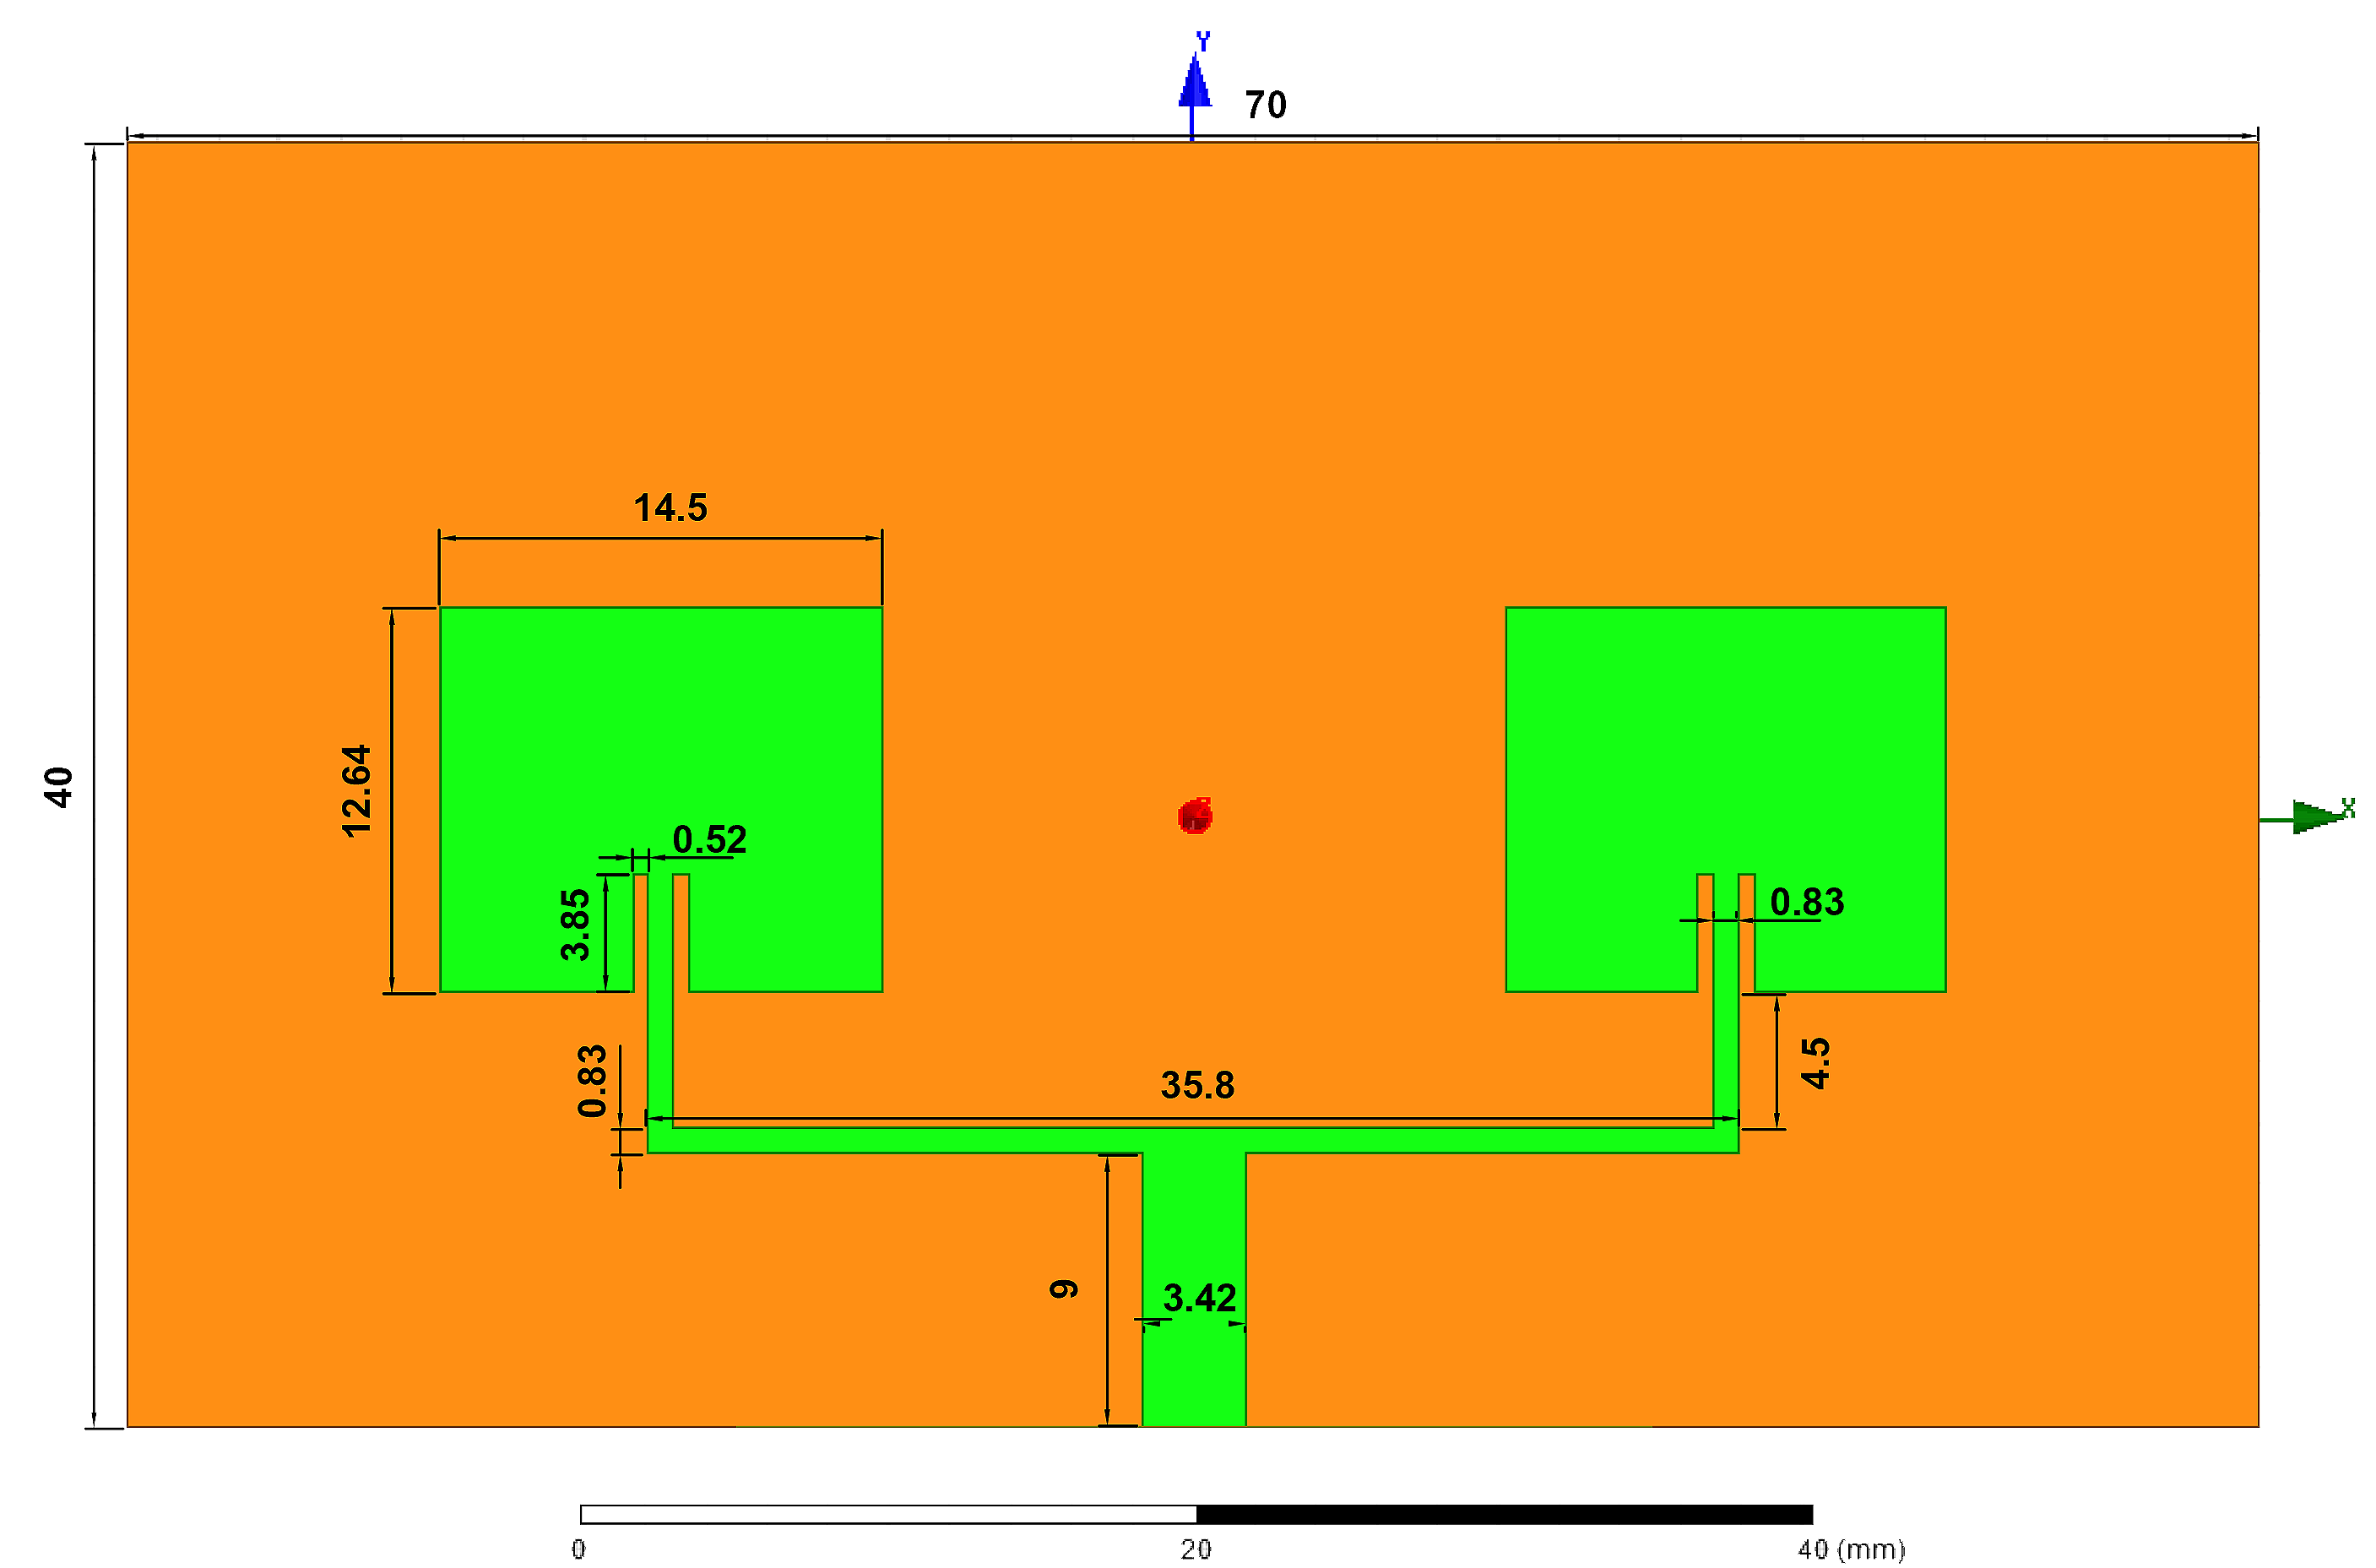
\includegraphics[width=18cm ,height=\textheight, keepaspectratio=true,angle=90,origin=c]{archivos/desarrollo/autocad/4}
        \caption{Dimensiones del array 2x1 a 6 GHz}
        \label{fig:2x12}
\end{figure}
\vfill
\textit{\textbf{Nota}}: todas las medidas están expresadas en milímetros.
\newpage

\section{Array 2x2 @ 2.4 GHz}
\vfill
\begin{figure}[H]
   	 \centering
        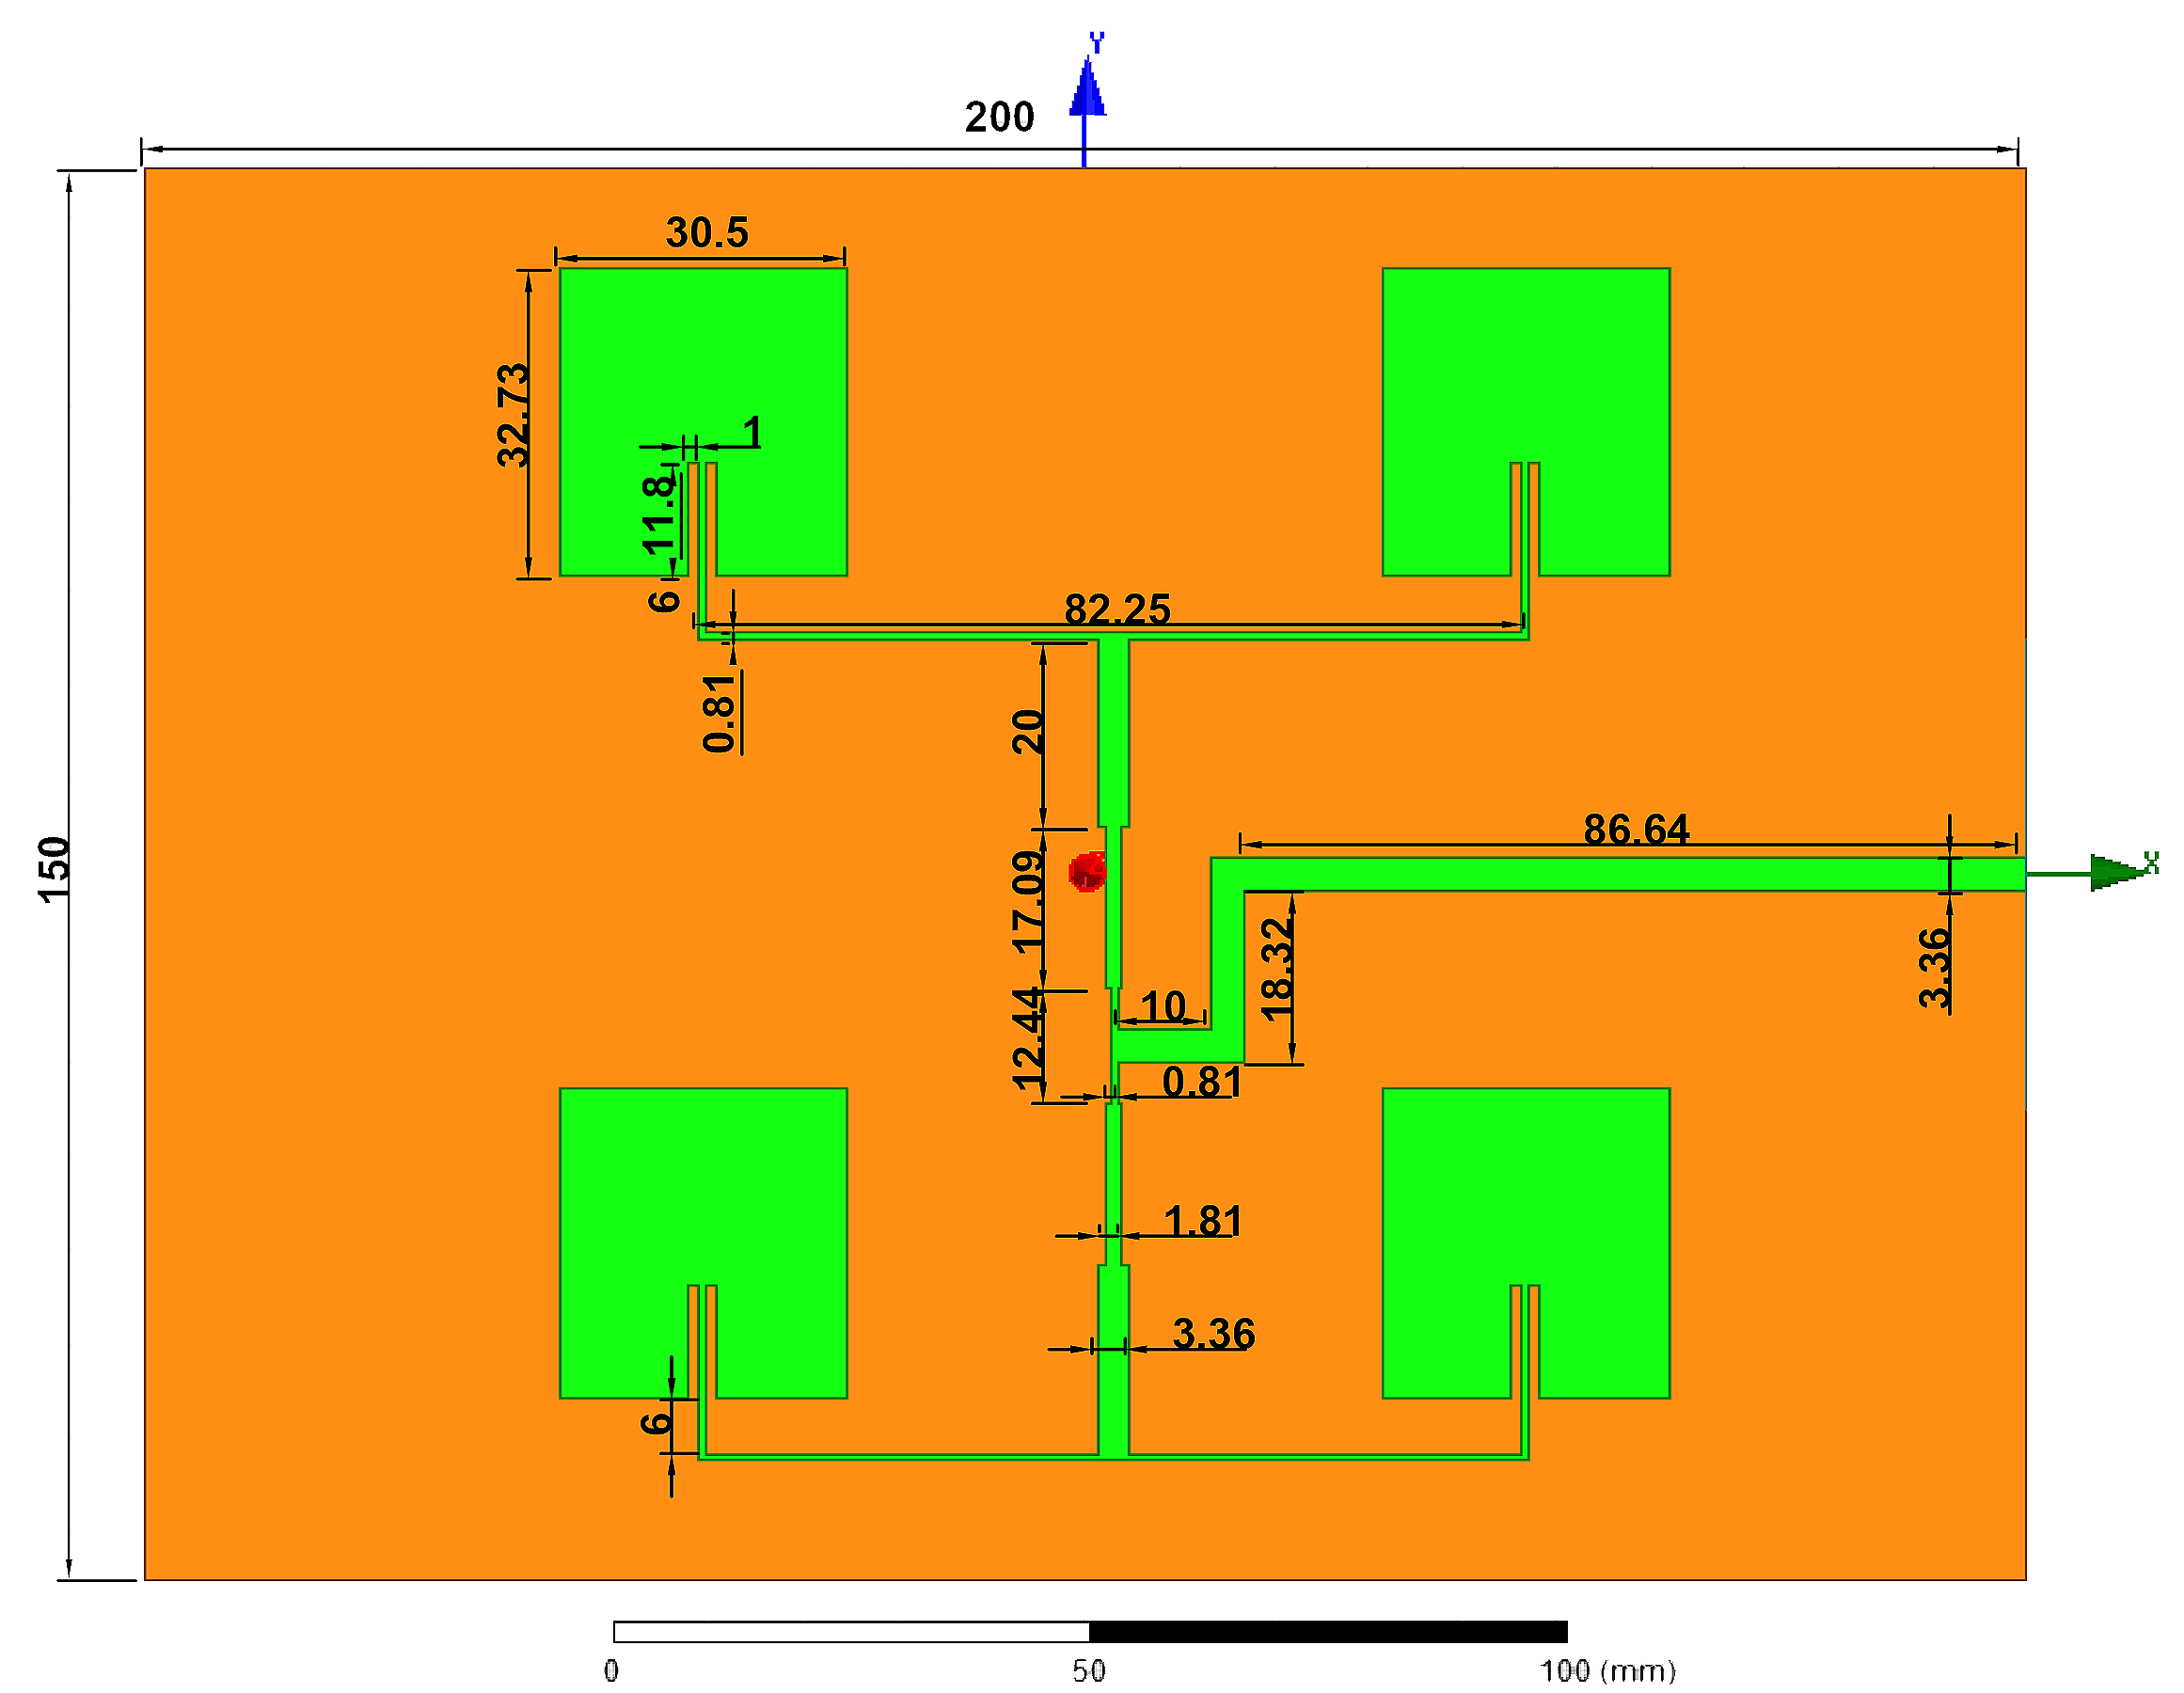
\includegraphics[width=\textwidth ,height=\textheight, keepaspectratio=true]{archivos/desarrollo/autocad/7}
        \caption{Dimensiones del array 2x2 a 2.4 GHz}
        \label{fig:2x21}
\end{figure}
\vfill
\textit{\textbf{Nota}}: todas las medidas están expresadas en milímetros.
\newpage

\section{Array 2x2 @ 6 GHz}
\vfill
\begin{figure}[H]
   	 \centering
        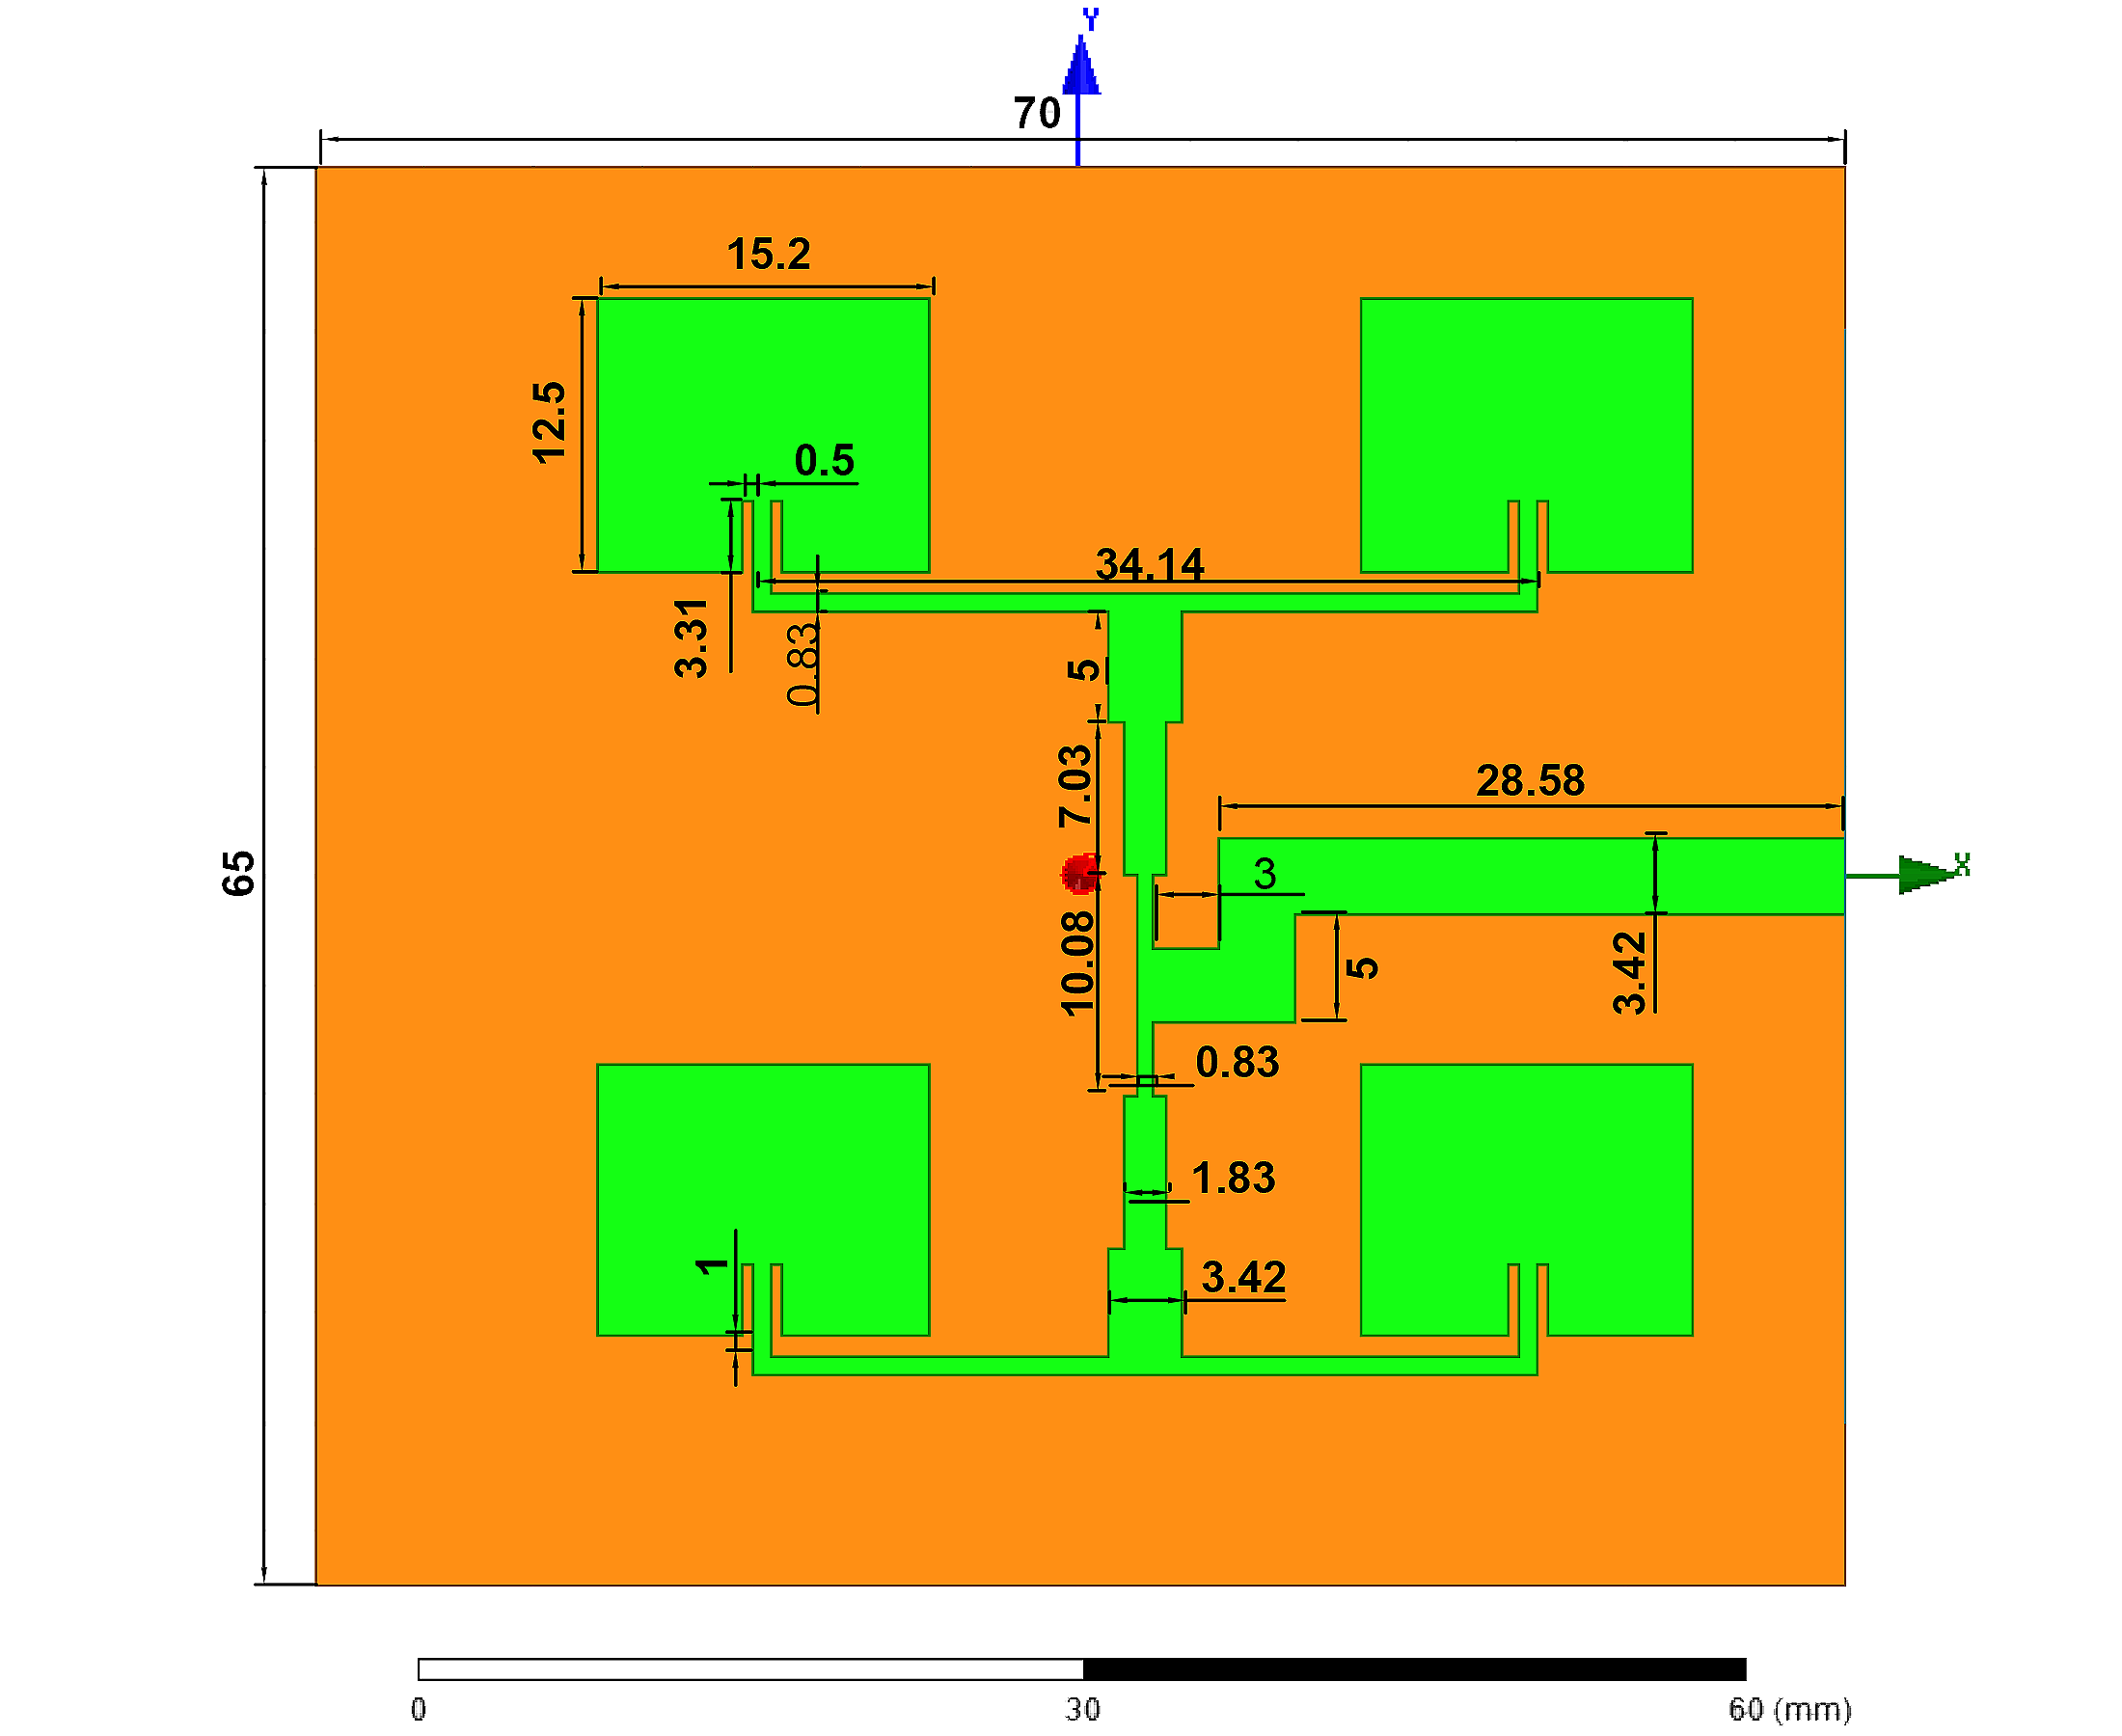
\includegraphics[width=\textwidth ,height=\textheight, keepaspectratio=true]{archivos/desarrollo/autocad/8}
        \caption{Dimensiones del array 2x2 a 6 GHz}
        \label{fig:2x22}
\end{figure}
\vfill
\textit{\textbf{Nota}}: todas las medidas están expresadas en milímetros.
\newpage

\section{Array 4x1 @ 2.4 GHz}
\vfill
\begin{figure}[H]
   	 \centering
        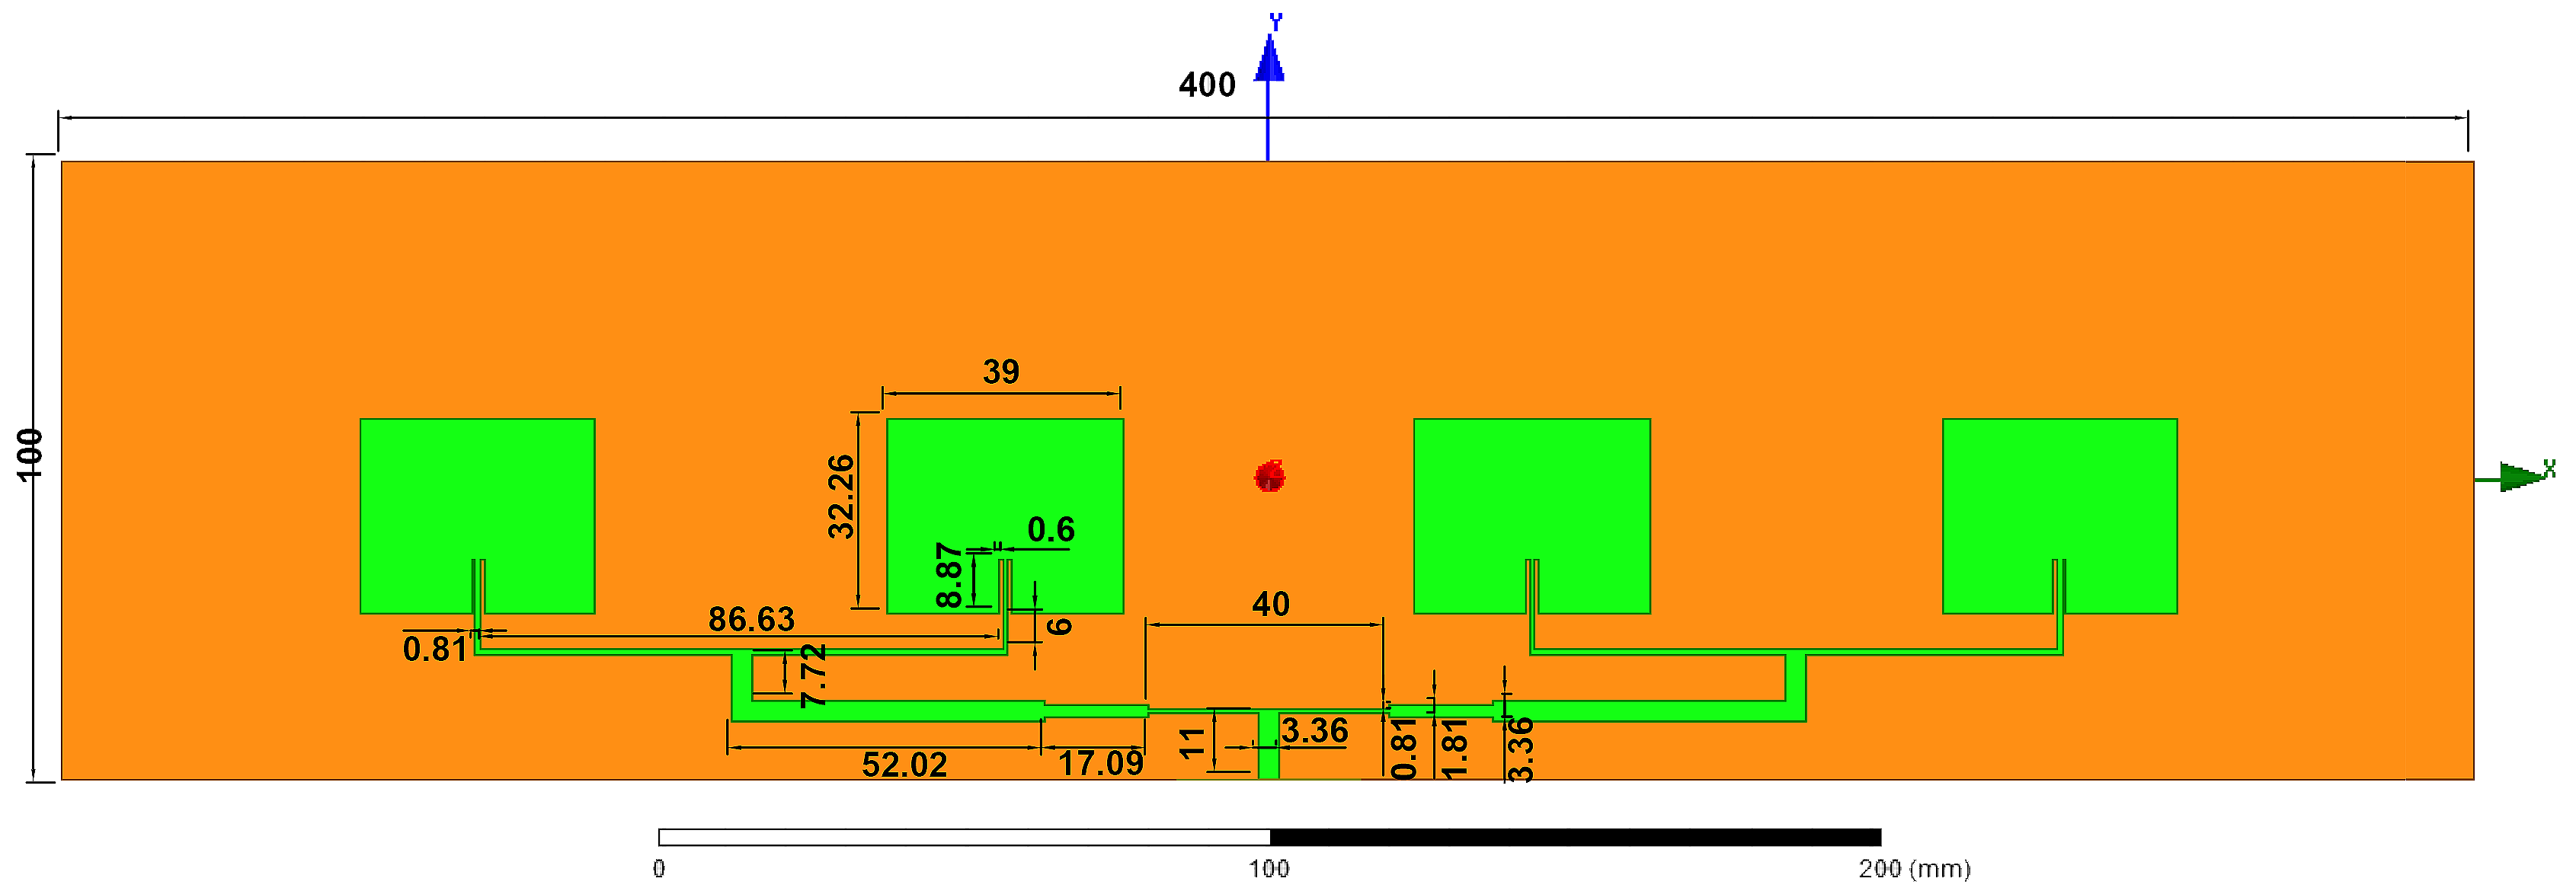
\includegraphics[width=18cm ,height=\textheight, keepaspectratio=true, angle=90,origin=c]{archivos/desarrollo/autocad/5}
        \caption{Dimensiones del array 4x1 a 2.4 GHz}
        \label{fig:4x11}
\end{figure}
\vfill
\textit{\textbf{Nota}}: todas las medidas están expresadas en milímetros.
\newpage

\section{Array 4x1 @ 6 GHz}
\vfill
\begin{figure}[H]
   	 \centering
        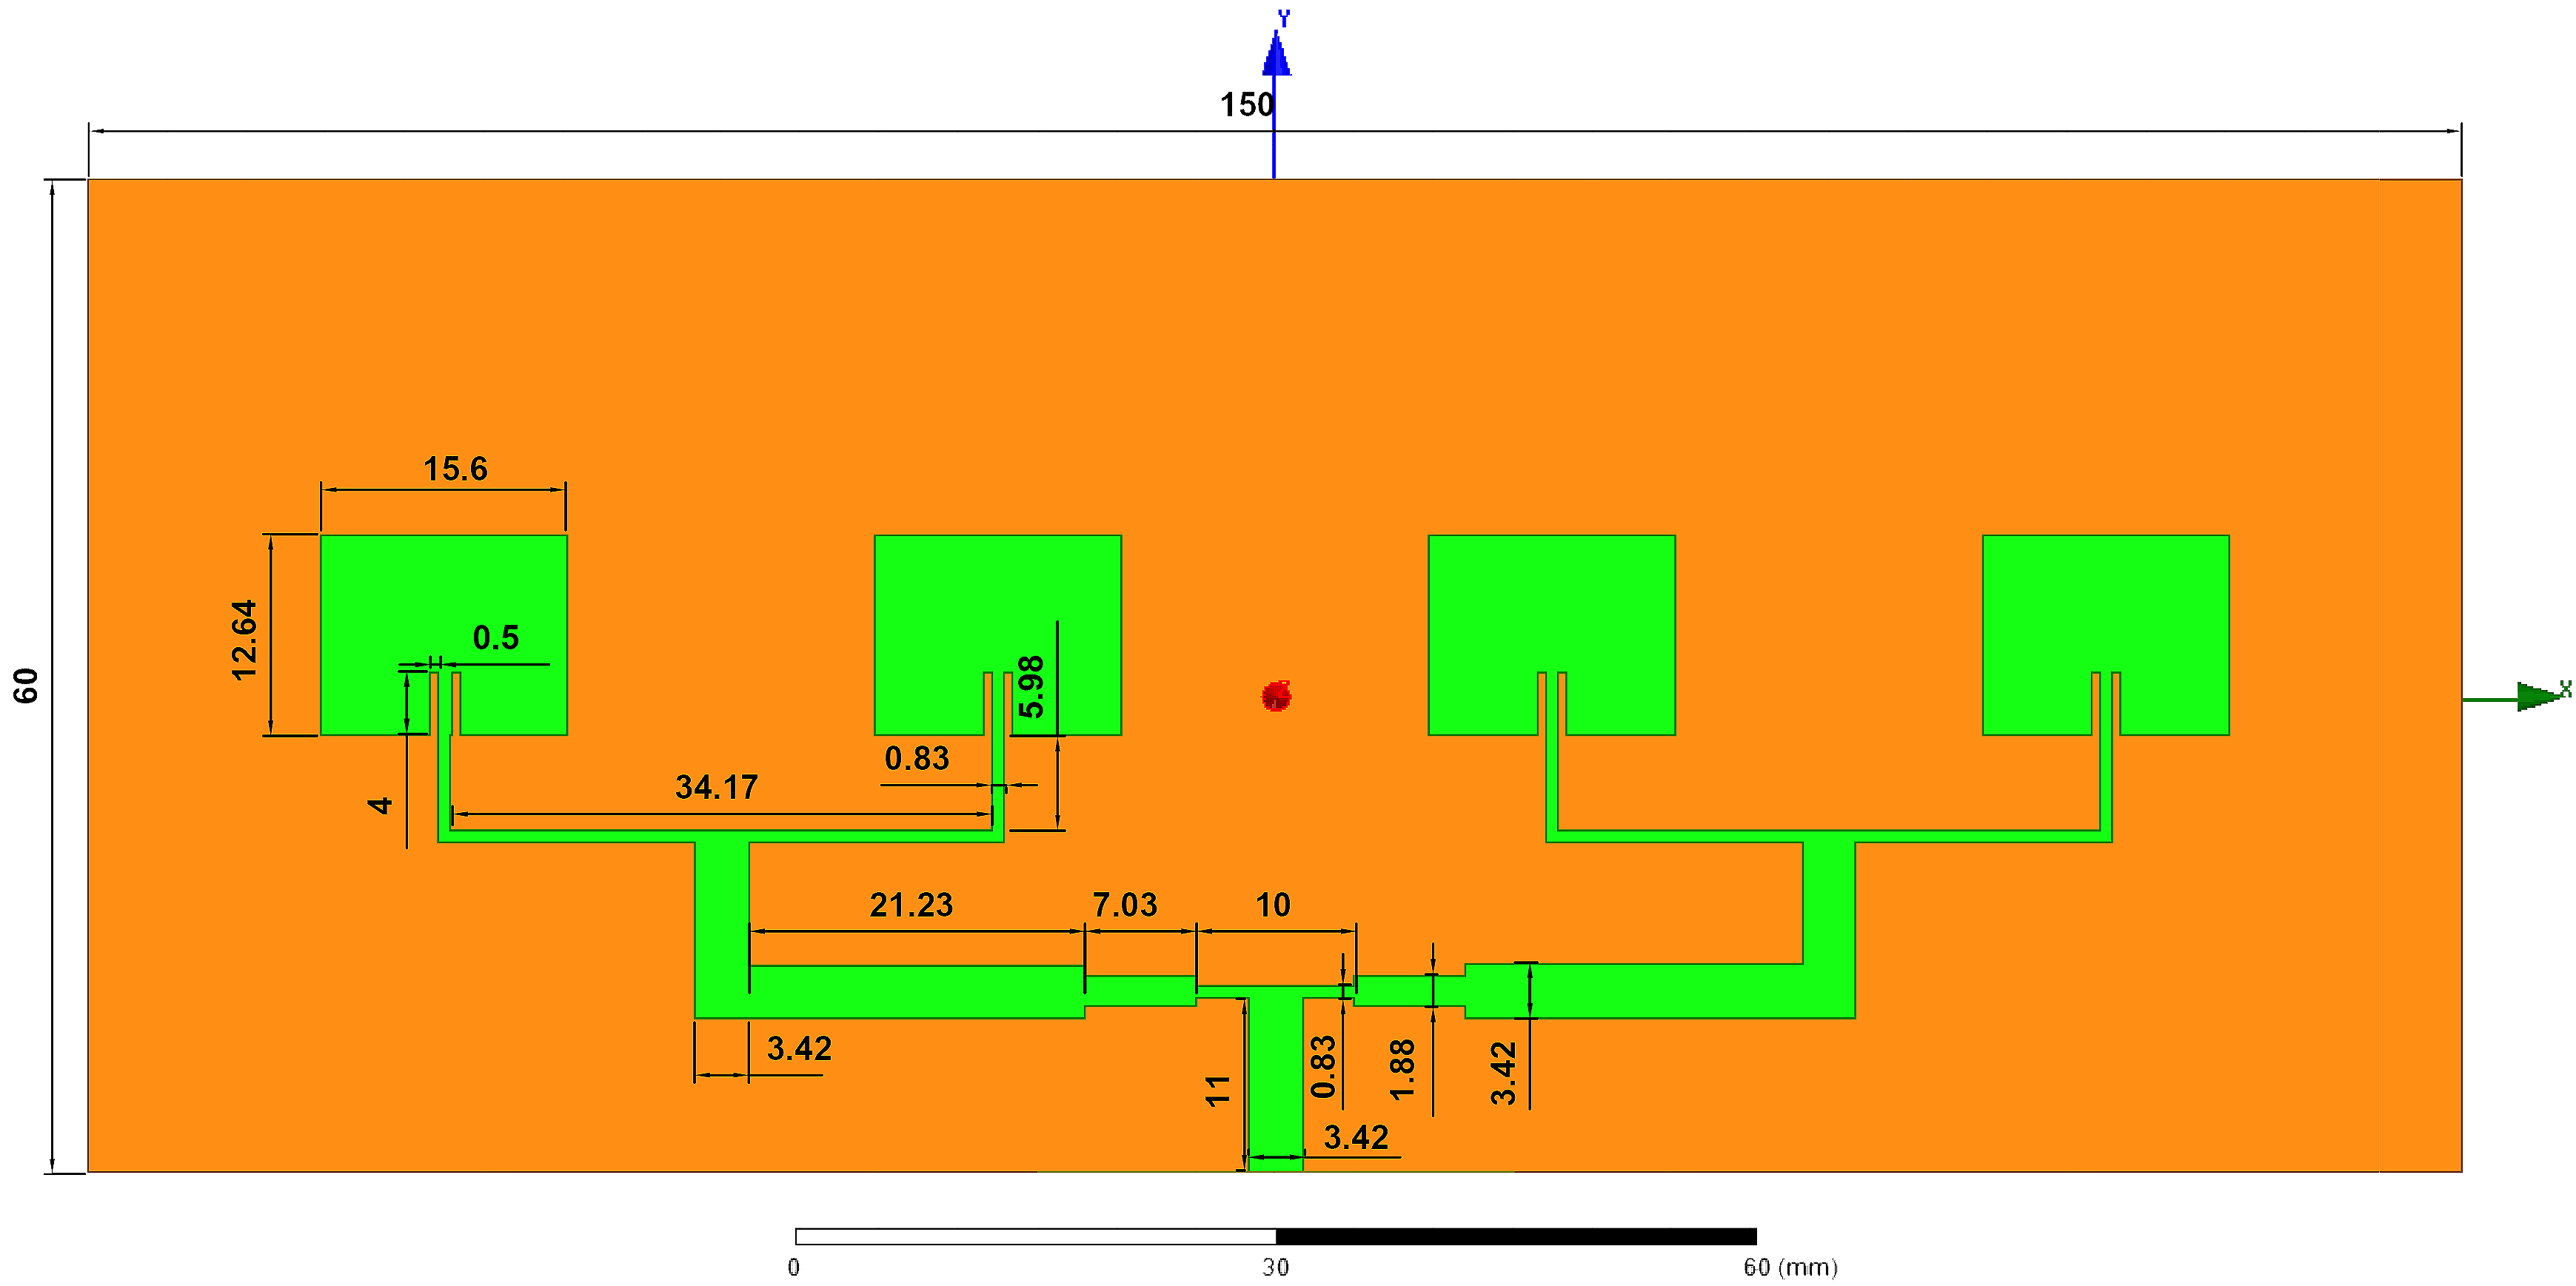
\includegraphics[width=18cm ,height=\textwidth, keepaspectratio=true, angle=90,origin=c]{archivos/desarrollo/autocad/6}
        \caption{Dimensiones del array 4x1 a 6 GHz}
        \label{fig:4x12}
\end{figure}
\vfill
\textit{\textbf{Nota}}: todas las medidas están expresadas en milímetros.
\newpage

\section{Array 4x2 @ 2.4 GHz}
\vfill
\begin{figure}[H]
   	 \centering
        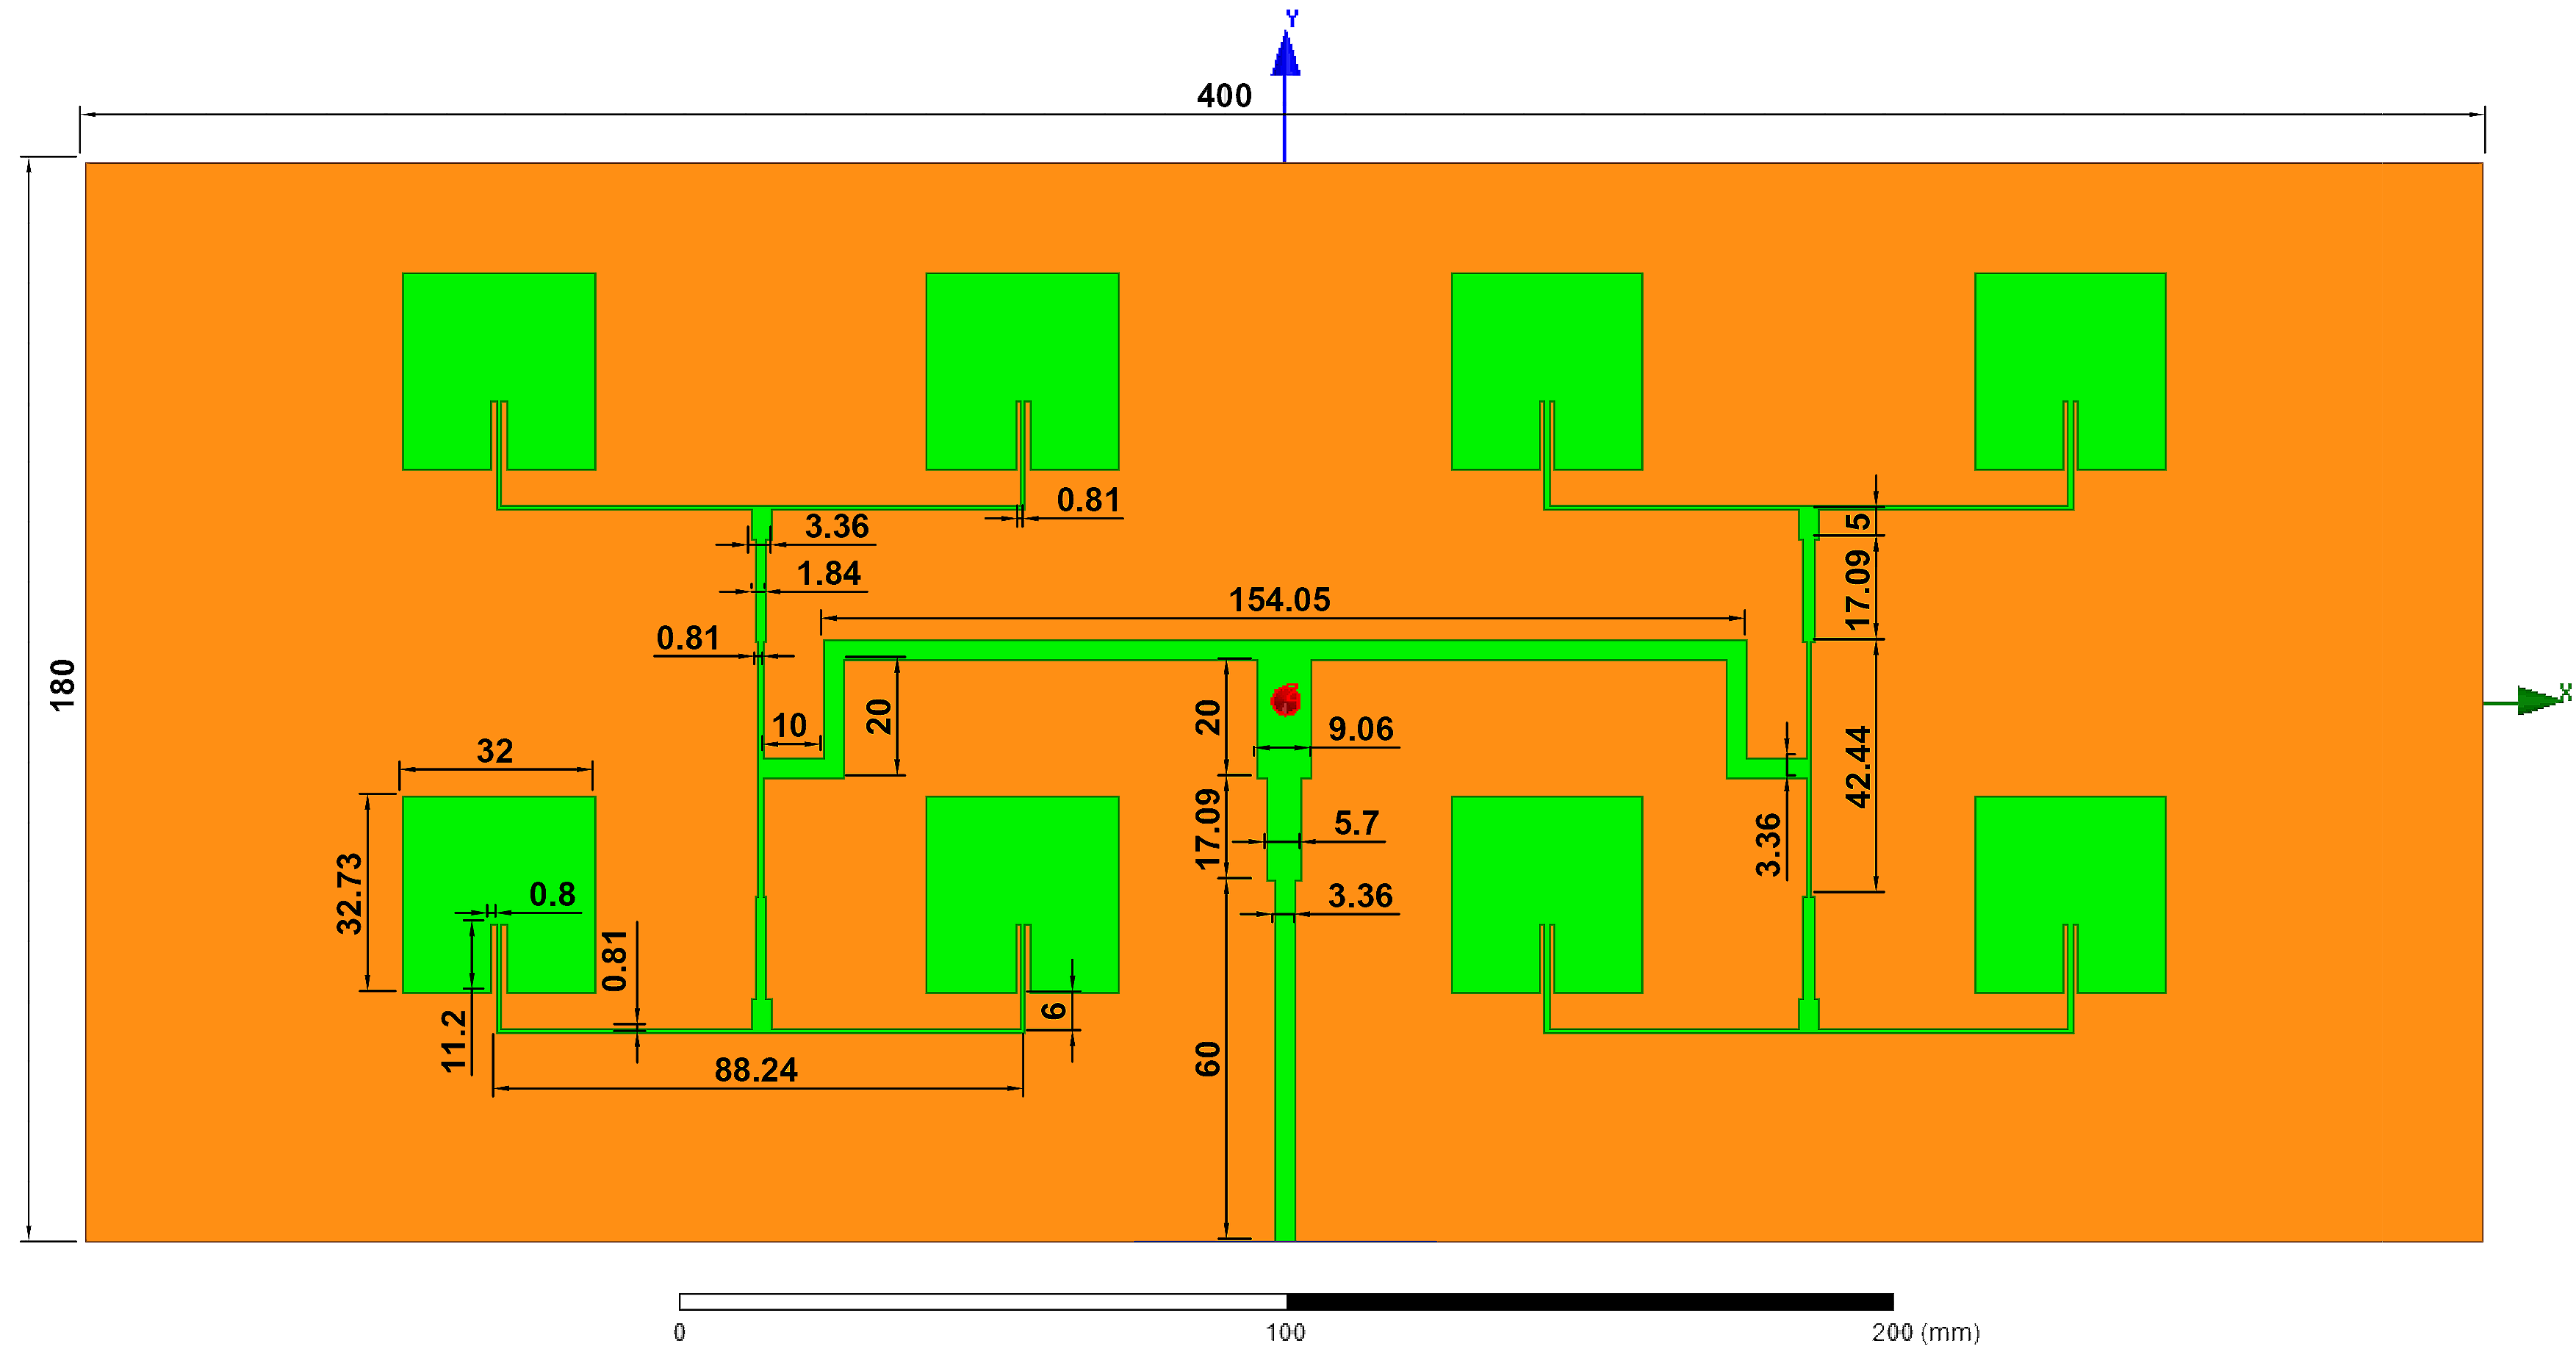
\includegraphics[width=18cm ,height=\textwidth, keepaspectratio=true, angle=90,origin=c]{archivos/desarrollo/autocad/9}
        \caption{Dimensiones del array 4x2 a 2.4 GHz}
        \label{fig:4x21}
\end{figure}

\vfill
\textit{\textbf{Nota}}: todas las medidas están expresadas en milímetros.
\newpage

\section{Array 4x4 @ 2.4 GHz}
\vfill
\begin{figure}[H]
   	 \centering
        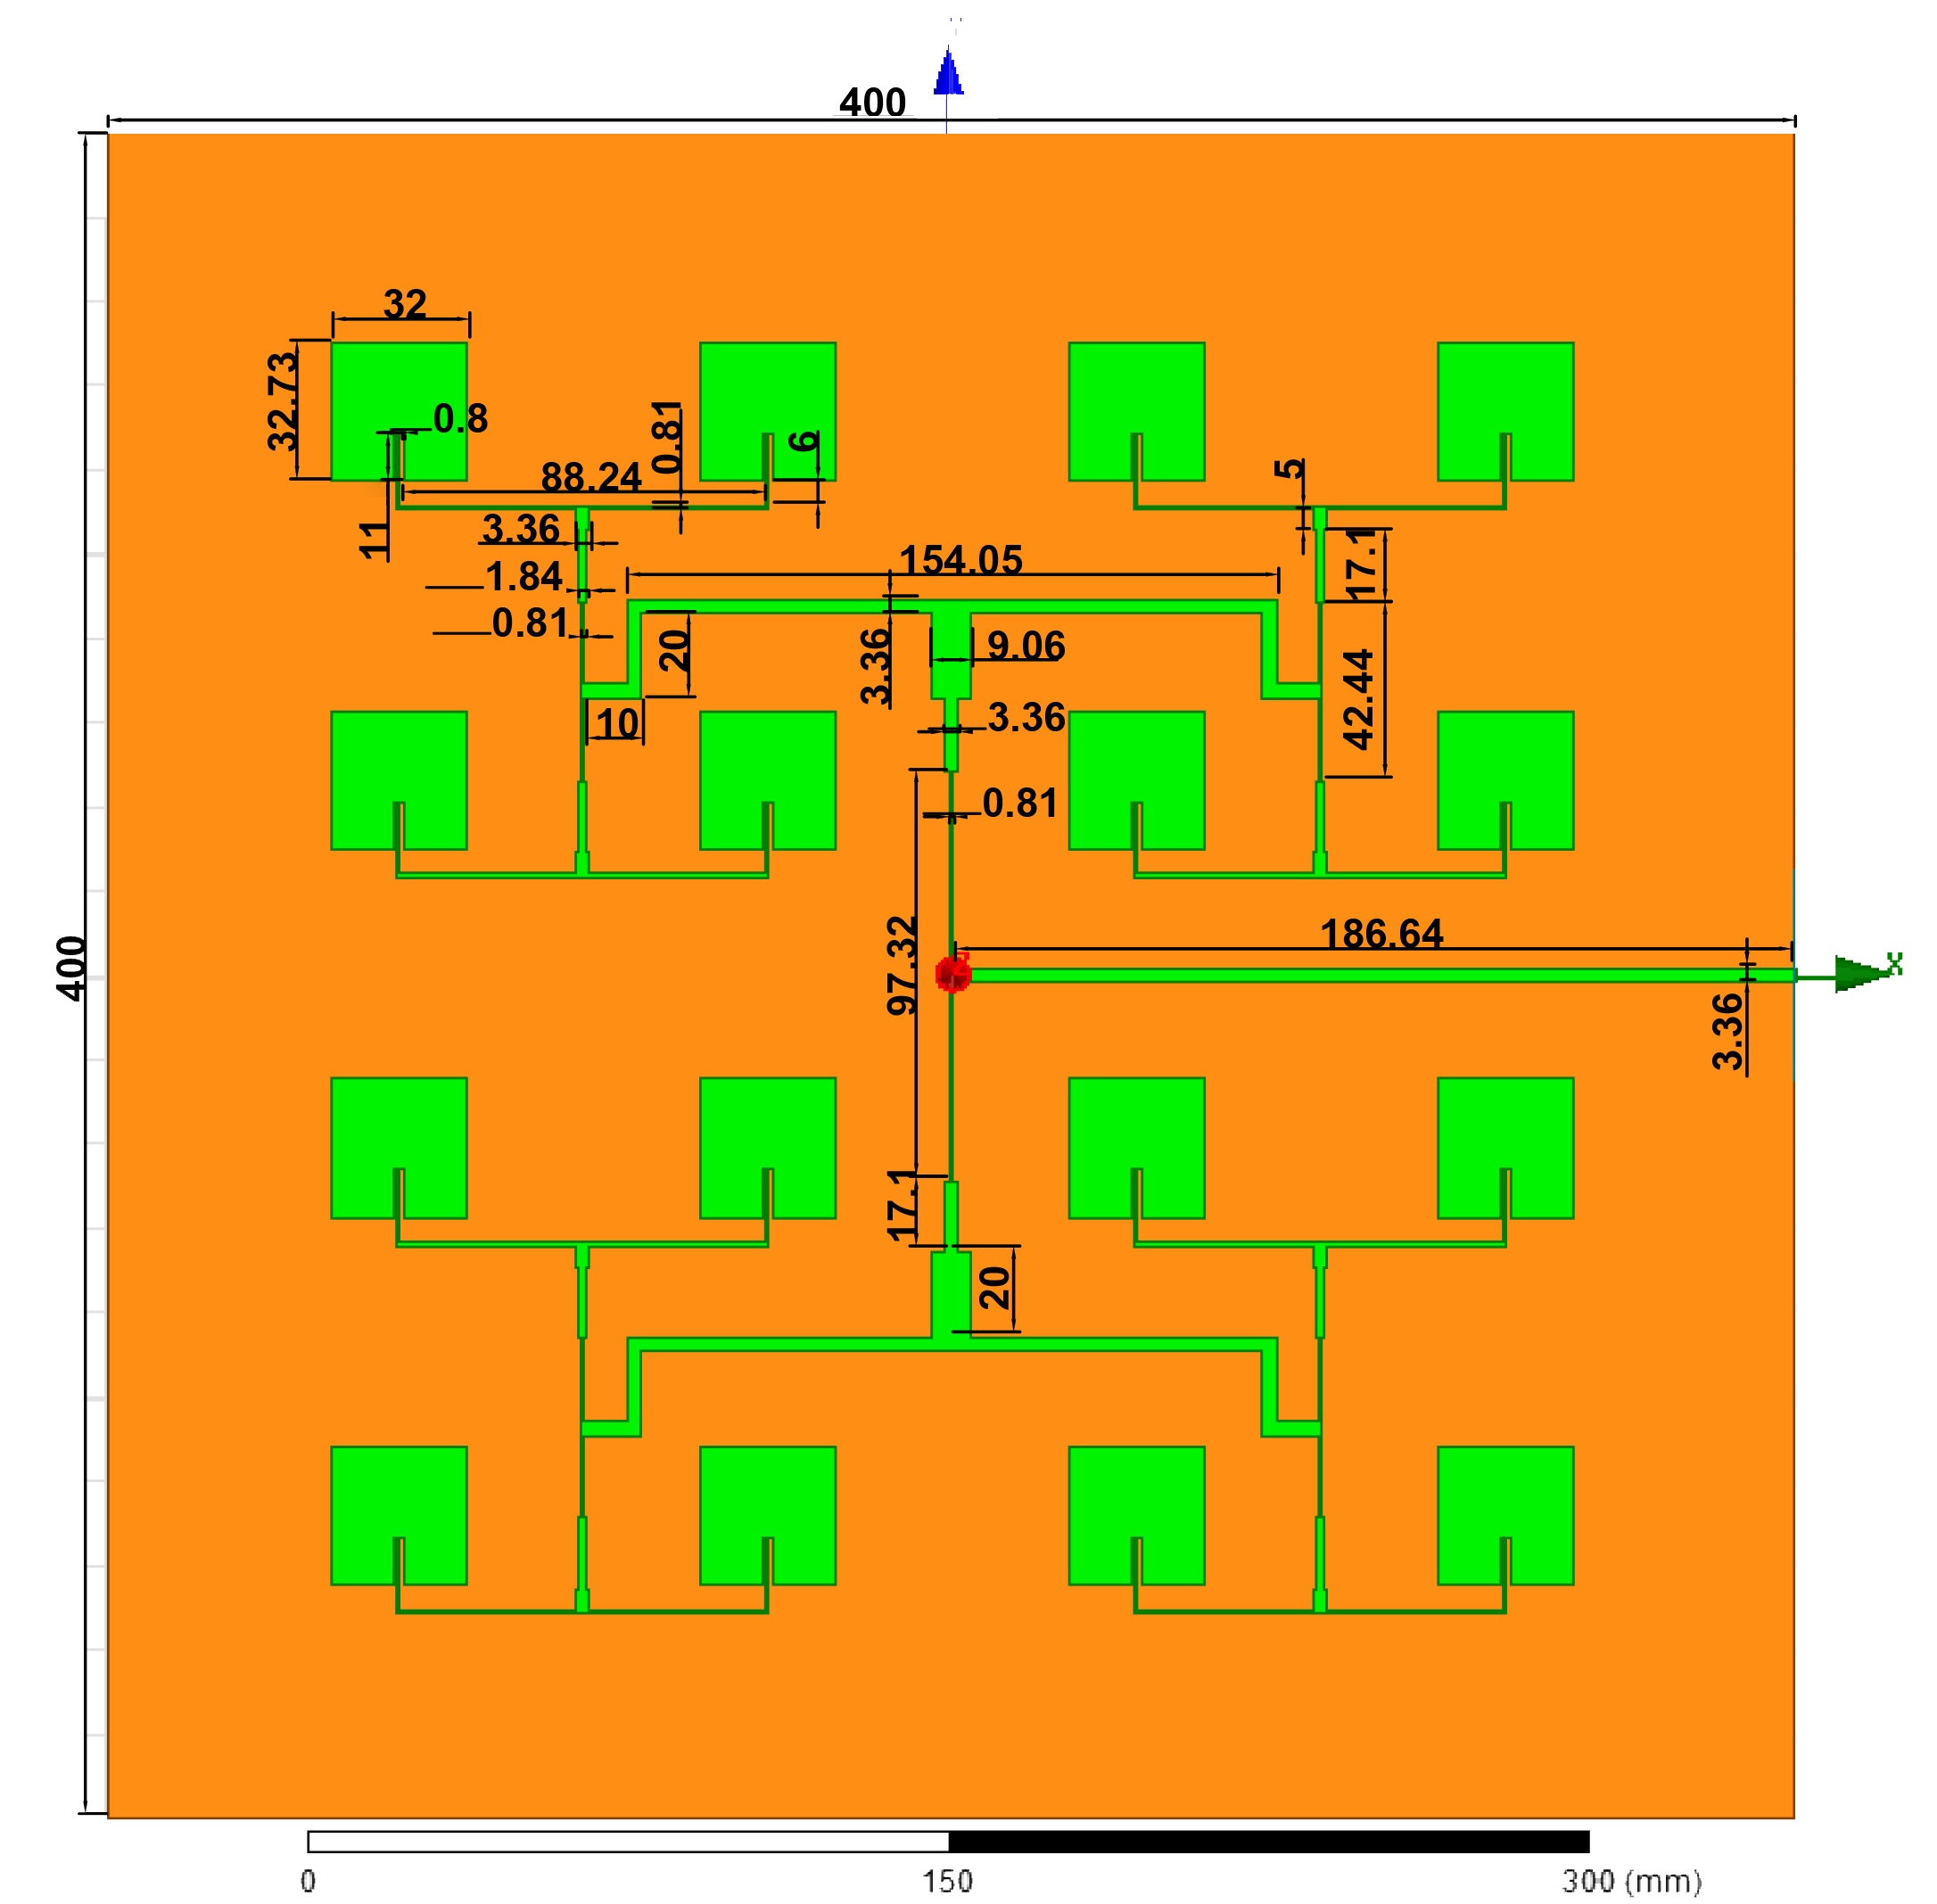
\includegraphics[width=\textwidth ,height=\textheight, keepaspectratio=true]{archivos/desarrollo/autocad/10}
        \caption{Dimensiones del array 4x4 a 2.4 GHz}
        \label{fig:4x41}
\end{figure}
\vfill
\textit{\textbf{Nota}}: todas las medidas están expresadas en milímetros.
\newpage


\section{Array 4x4 @ 6 GHz}
\vfill
\begin{figure}[H]
   	 \centering
        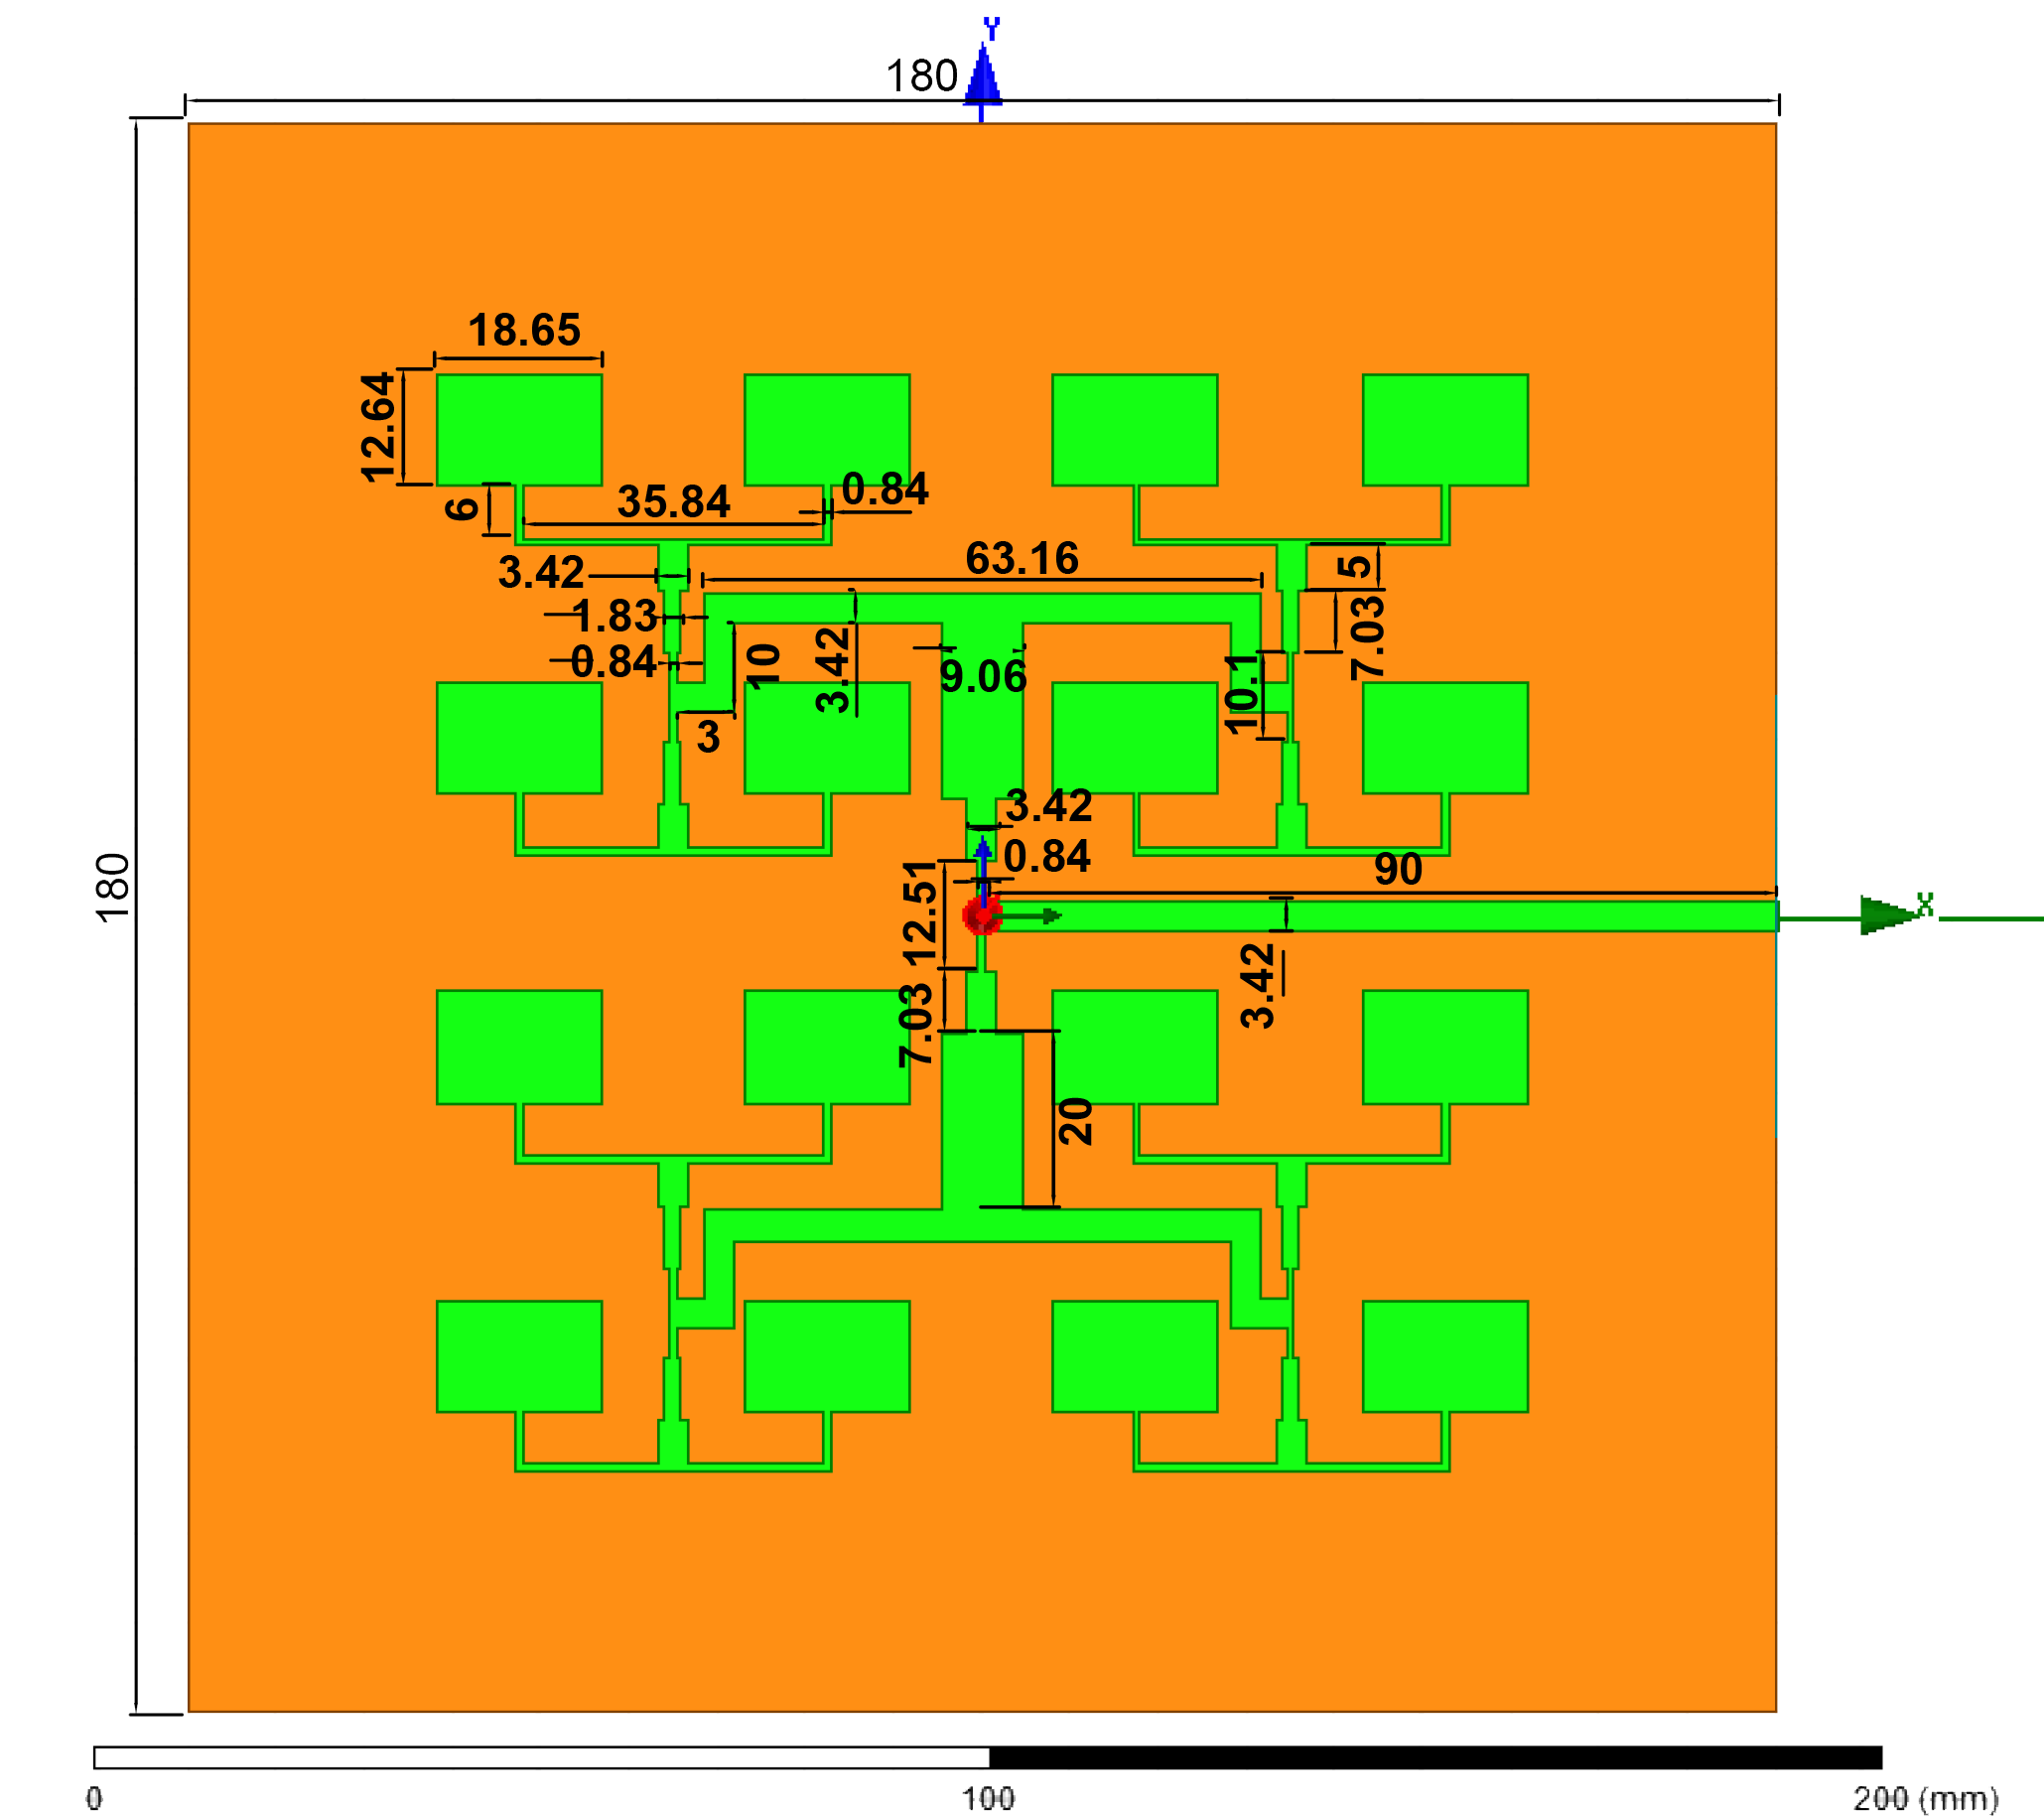
\includegraphics[width=\textwidth ,height=\textheight, keepaspectratio=true]{archivos/desarrollo/autocad/11}
        \caption{Dimensiones del array 4x4 a 6 GHz}
        \label{fig:4x42}
\end{figure}
\vfill
\textit{\textbf{Nota}}: todas las medidas están expresadas en milímetros.
\newpage

\section{Parche Simple @ 27 GHz}
\vfill
\begin{figure}[H]
   	 \centering
        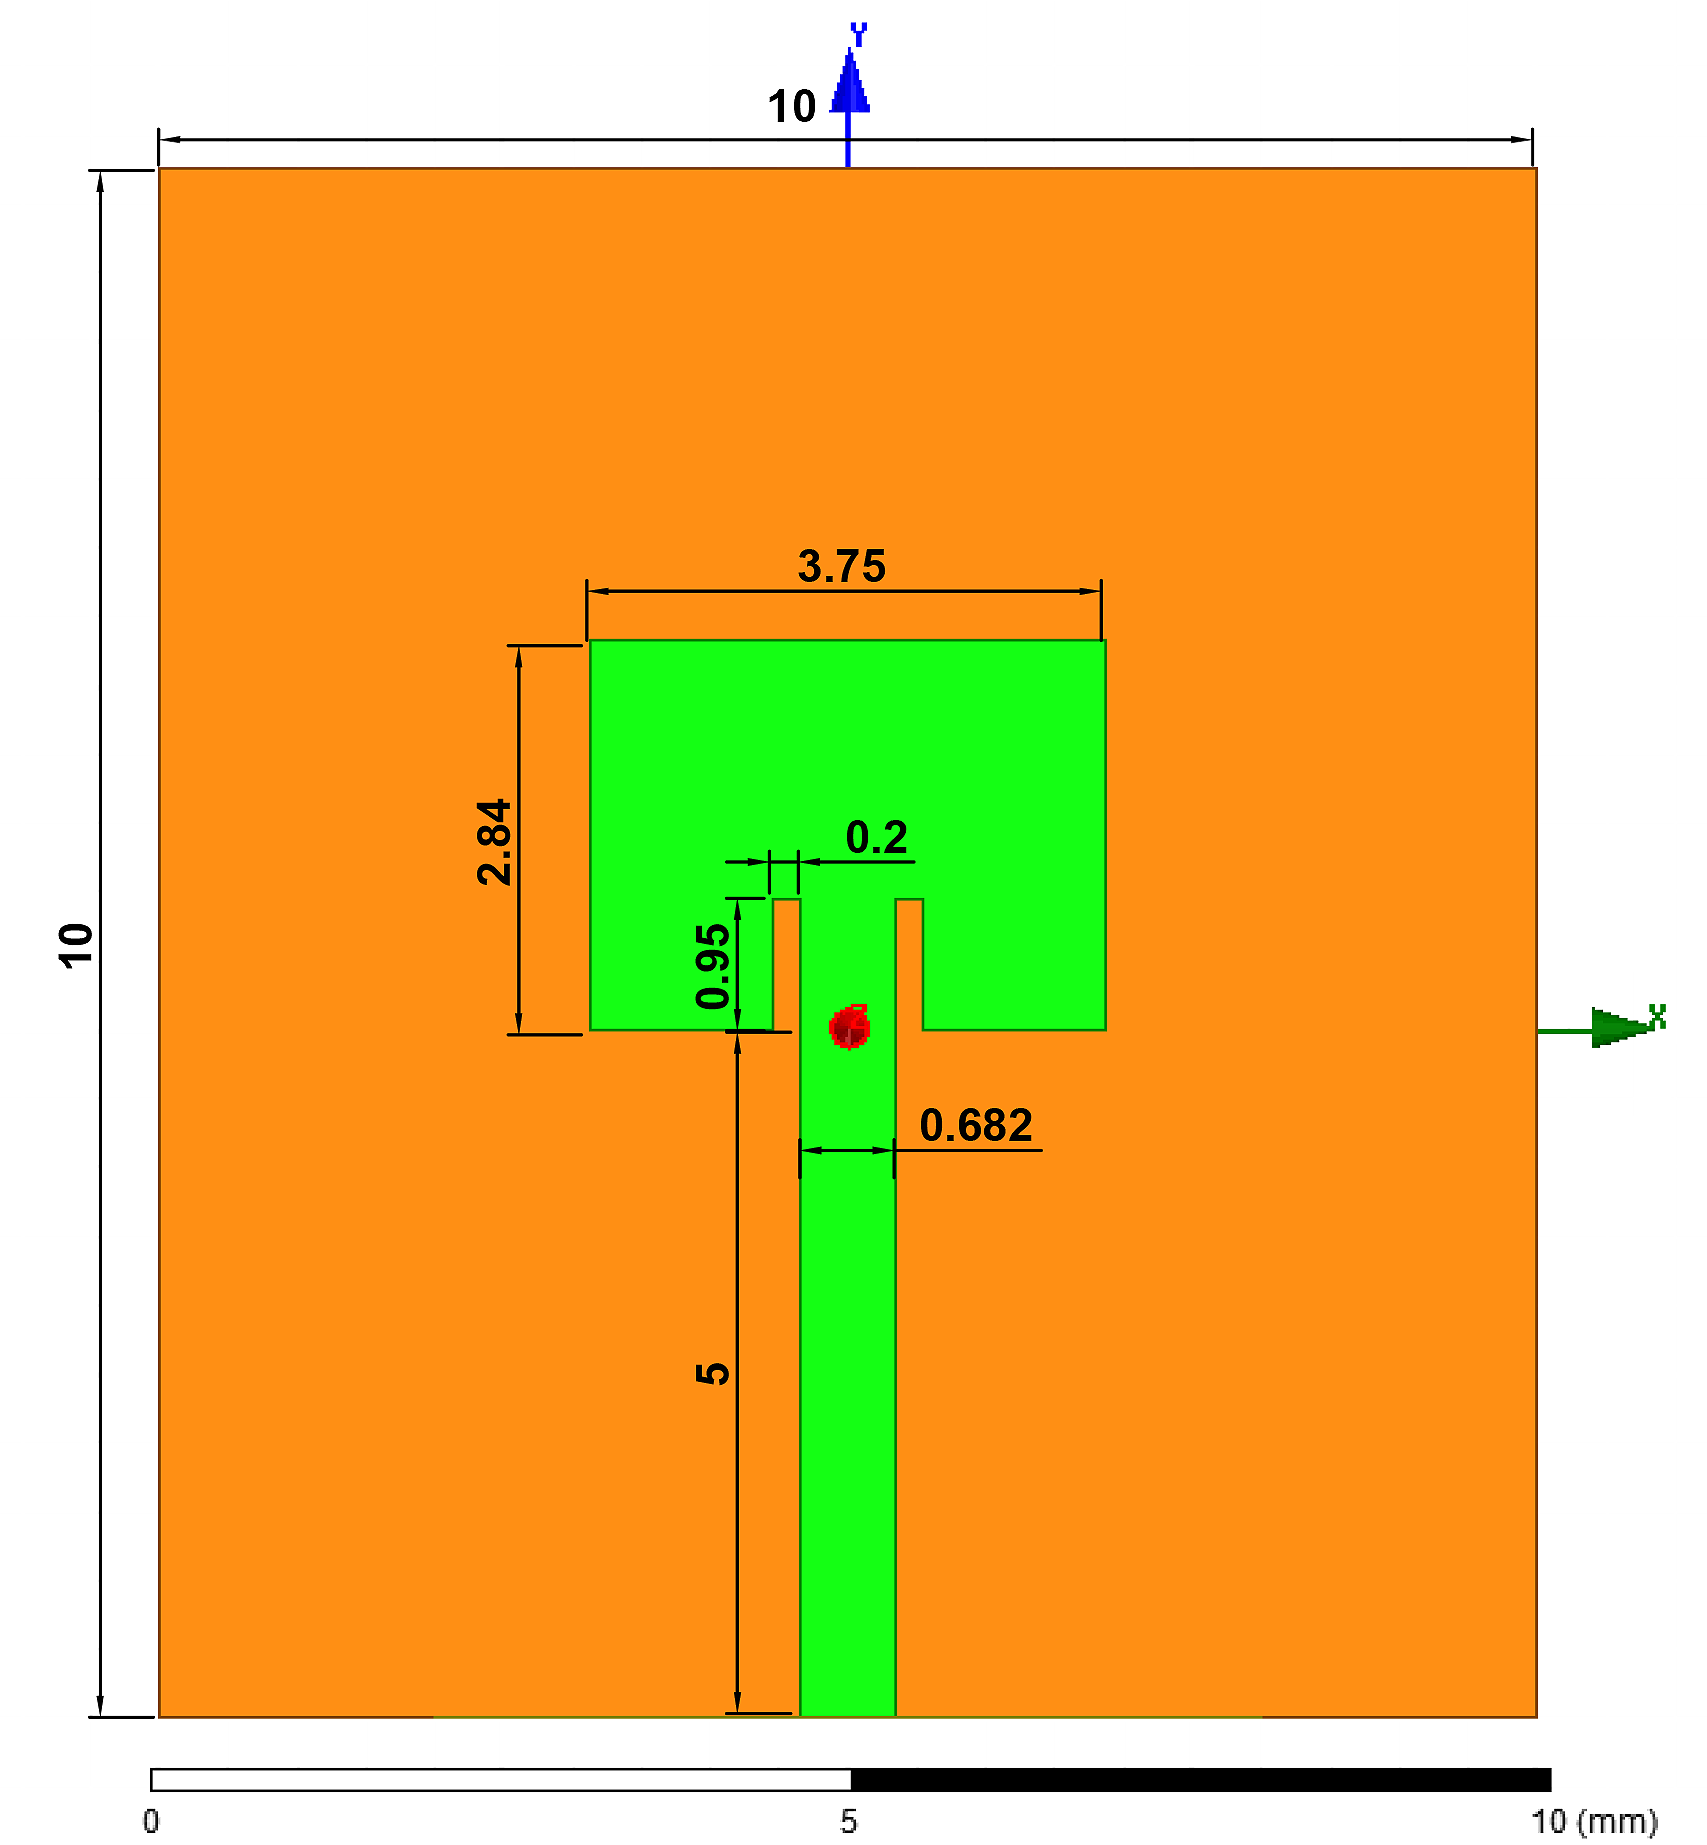
\includegraphics[width=\textwidth ,height=\textheight, keepaspectratio=true]{archivos/desarrollo/autocad/12}
        \caption{Dimensiones del parche simple a 27 GHz}
        \label{fig:1x13}
\end{figure}
\vfill
\textit{\textbf{Nota}}: todas las medidas están expresadas en milímetros.

\section{Array 2x1 @ 27 GHz}
\vfill
\begin{figure}[H]
   	 \centering
        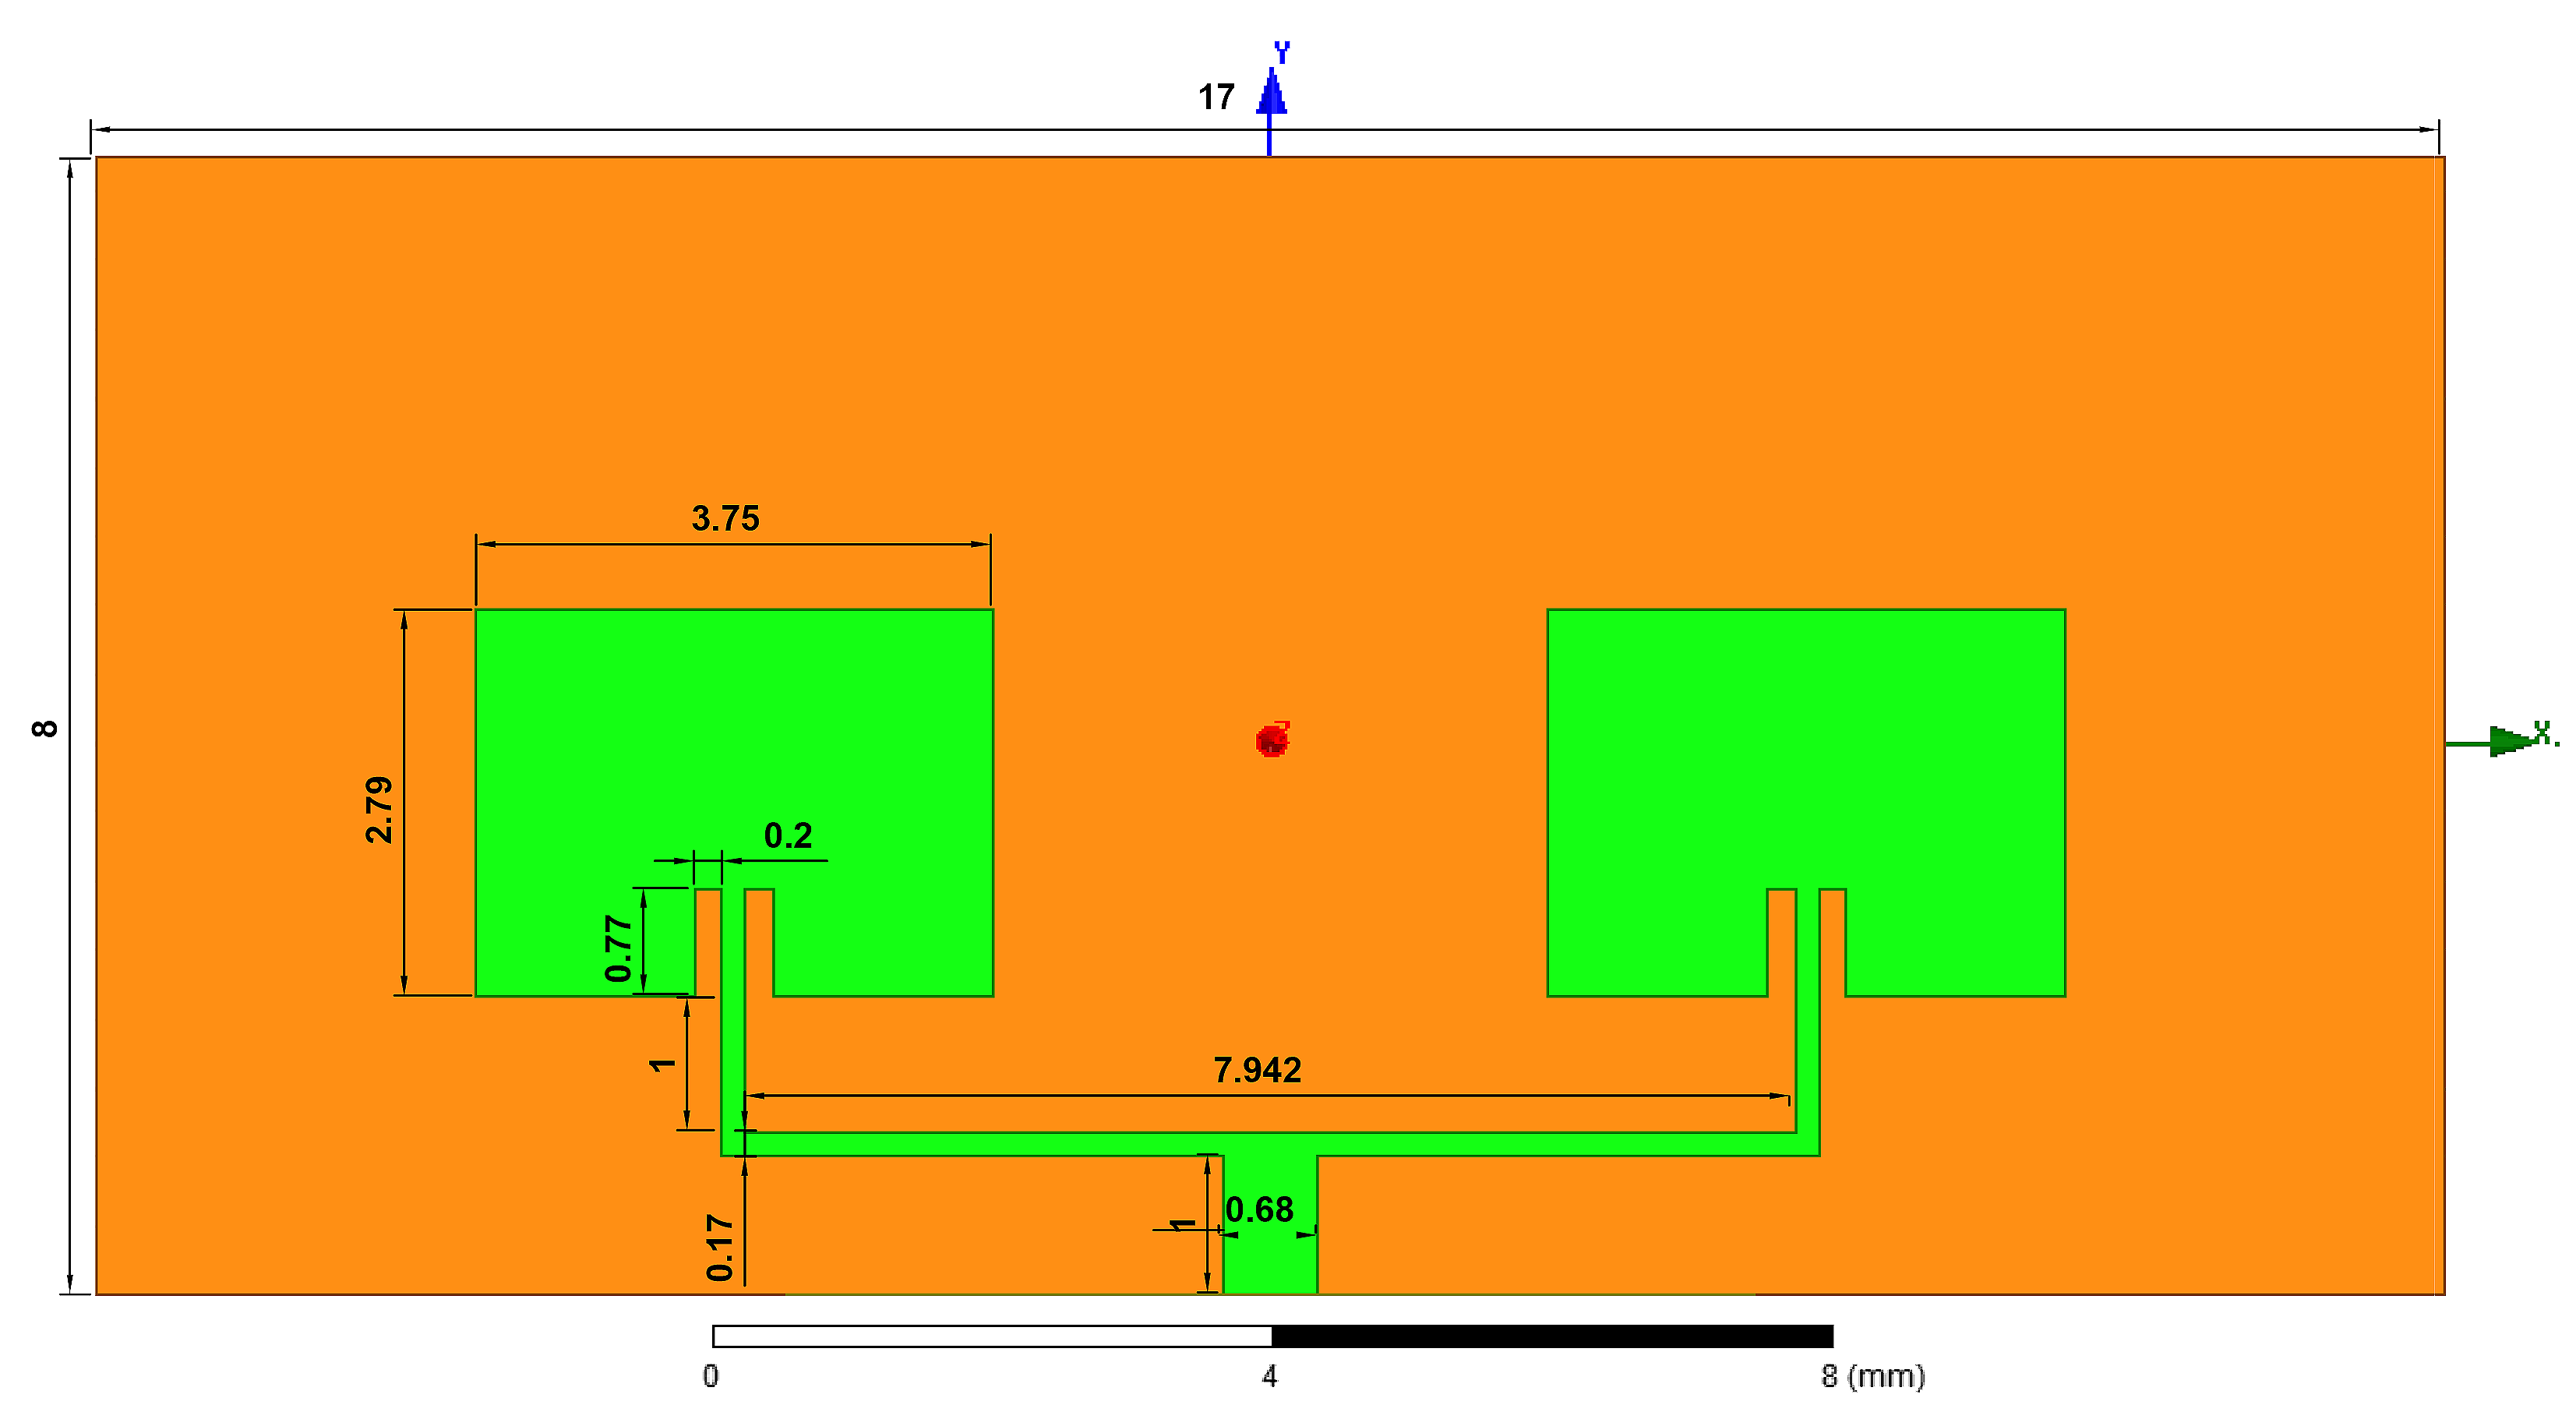
\includegraphics[width=\textwidth ,height=\textheight, keepaspectratio=true,angle=90,origin=c]{archivos/desarrollo/autocad/13}
        \caption{Dimensiones del array 2x1 a 27 GHz}
        \label{fig:2x13}
\end{figure}
\vfill
\textit{\textbf{Nota}}: todas las medidas están expresadas en milímetros.


\section{Array 2x2 @ 27 GHz}
\vfill
\begin{figure}[H]
   	 \centering
        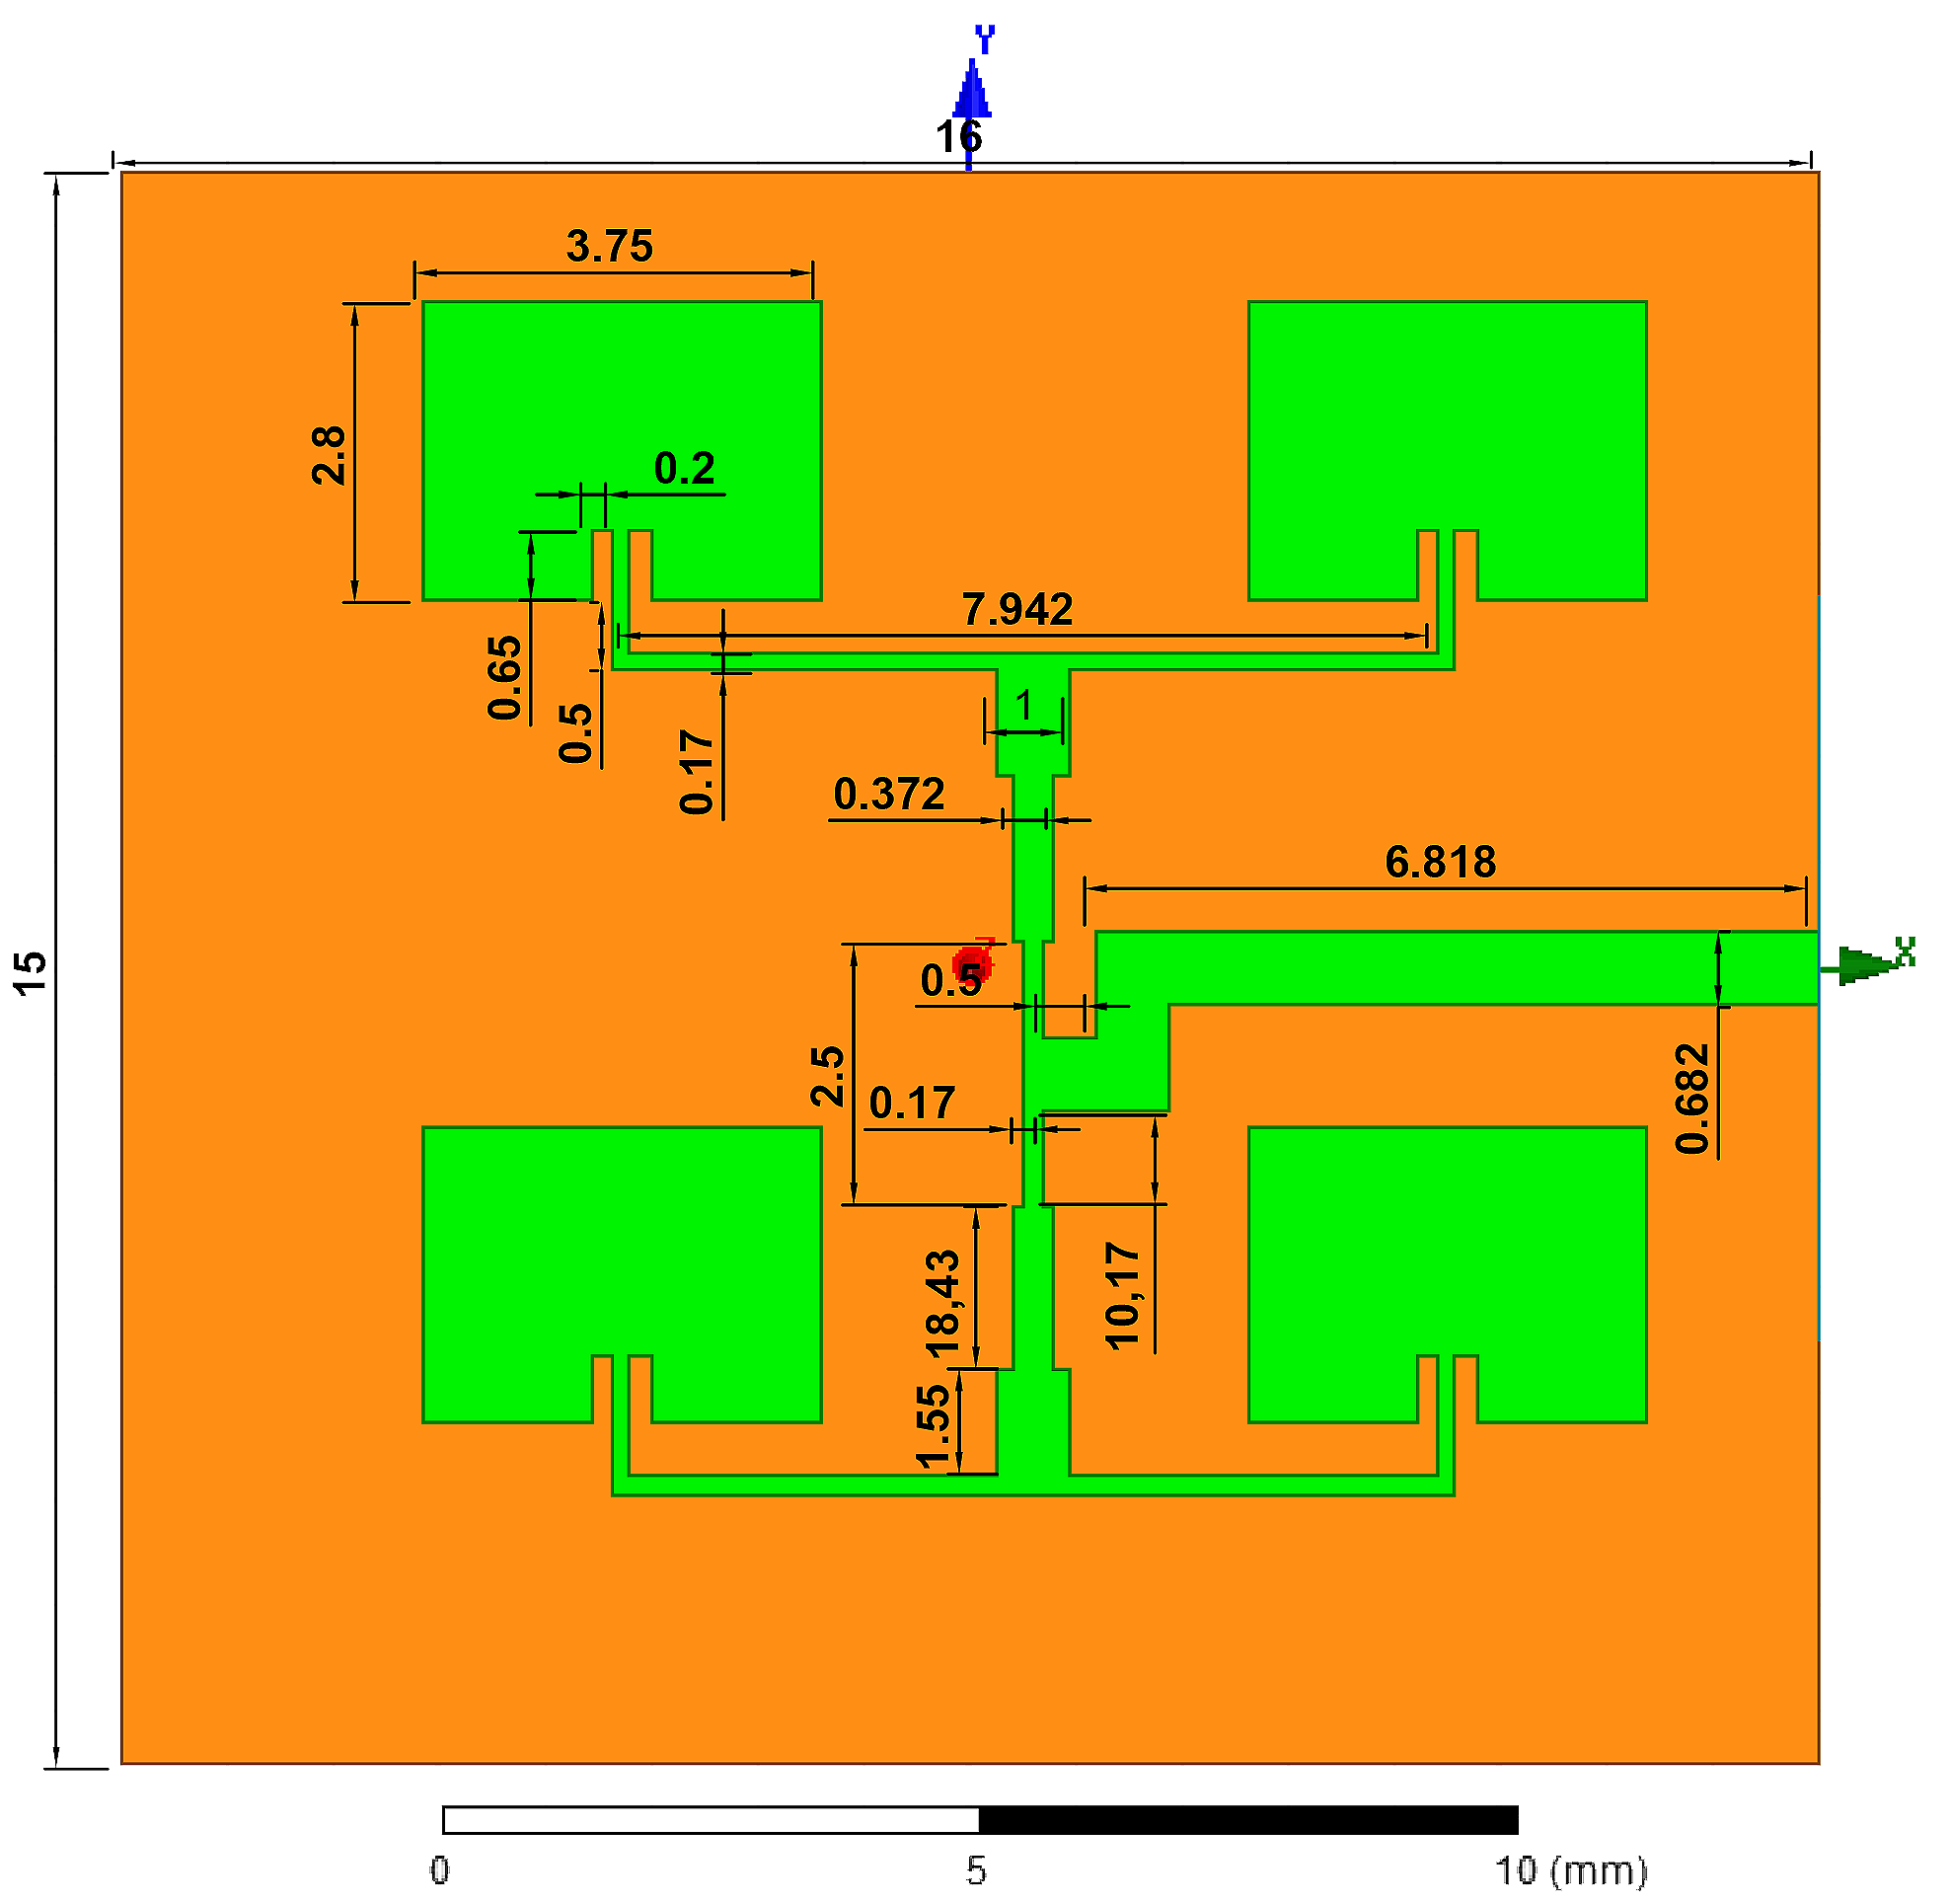
\includegraphics[width=\textwidth ,height=\textheight, keepaspectratio=true]{archivos/desarrollo/autocad/14}
        \caption{Dimensiones del array 2x2 a 27 GHz}
        \label{fig:2x23}
\end{figure}
\vfill
\textit{\textbf{Nota}}: todas las medidas están expresadas en milímetros.